\graphicspath{ {sections/} }

\chapter{Simulations on Optimal Auctions in Multidimensional Settings}\label{ch_auctions}I explore the properties of optimal multi-dimensional auctions in a setting where a single object of multiple qualities is sold to several buyers. Using simulations, I test the hypothesis that the optimal mechanism is an \textit{exclusive buyer mechanism}, where buyers compete to be the right to be the only buyer to choose between quality levels of a good. I find compelling evidence of the optimality of the exclusive buyer mechanism in multi-dimensional settings and explore other conjectures concerning the set of types excluded from the mechanism in equilibrium in optimal multidimensional auctions.

\section{Introduction}

Since the seminal work of Roger Myerson \autocite*{myerson1981optimal}, revenue-maximizing auctions in the case of a single dimension (e.g., good) are well known. However, little is known about optimal auctions in settings with multiple dimensions of value. The problem is incredibly complex: despite sustained research efforts for decades, only in the past few years have we discovered how to optimally sell two goods to a single buyer \autocite{daskalakis2017strong}. In this chapter, I focus on the multidimensional setting of a single good with multiple quality levels and explore whether a specific mechanism---the \textit{exclusive buyer mechanism}---is optimal. Building off existing work at the intersection of economics and computer science, I adopt a novel approach involving extensive simulations to explore the optimality of this particular mechanism. The approach adopted here makes use of a new approximation algorithm to uncover the qualitative features of optimal mechanisms in the particular multidimensional setting of a single good with multiple quality levels\footnote{The codebase for this project is available at \texttt{https://github.com/jmemich/optimal-auction-multidim}.}.

The setting of a single good with multiple quality levels can be understood as corresponding to the case of purchasing a single airplane ticket where the `quality level' might be: economy class, business class, or first class. A buyer might prefer, say, business over economy class. Each quality level can be (and very often is) given a different price and might have different value to the buyer. Crucially, unlike the multidimensional setting where multiple goods are sold by a seller to an arbitrary number of buyers, here since only one good is sold so `bundling'---selling subsets of all offered goods for a discount---cannot occur. The absence of bundling renders this a much simpler setting and an ideal point of departure for investigating the qualitative features of optimal multidimensional auctions.

In this thesis chapter, I am particularly concerned with investigating the optimality of the exclusive buyer mechanism in the setting of selling a single good with multiple quality levels to multiple bidders. This mechanism can be understood as an (either a second price or ascending bid) auction with a reserve price for the exclusive right to be the buyer of one of the quality levels of the good. The intuition for why this mechanism might be optimal can be reduced to: when there is a single good for sale with multiple dimensions of value, it is enough to consider the bidder who values a single quality level more than any other bidder values any other quality level. The exclusive buyer mechanism has previously been explored in multidimensional settings (e.g., \cite{brusco2011, belloni2010multidimensional}) but this thesis chapter represents the first sustained exploration of its optimality in a wide range of settings. This chapter develops the exclusive buyer mechanism in much broader generality, facilitating an extended investigation into its optimality in a broad range of multidimensional settings. 
 

% The exclusive buyer mechanism has previously been explored in multidimensional settings (e.g., \cite{brusco2011, belloni2010multidimensional}) but this thesis chapter represents the first sustained exploration of its optimality in a wide range of settings. This chapter first considers cases where significant prior research (of either analytic or computational character) exists. These settings are that of \autocite{pavlov2011optimal}, who conducted found the optimal mechanism for substitute goods in the case of a single buyer with symmetric, uniform valuations, and \autocite{belloni2010multidimensional}, who developed the original approximation algorithm for multidimensional settings when a single good with multiple quality levels is sold to an arbitrary number of buyers. Both of these settings consider cases where buyer's valuations across quality grades are independent and uniformly distributed. We extend the range of cases to those involving other types of distributions as well as arbitrary correlations across quality grades. Where computationally feasible, we consider settings where the number of buyers is greater than two.

The approach adopted in this chapter is to eschew analytic results in settings where few have been forthcoming in favor of exploring these complex, analytically intractable settings using simulations to approximate optimal mechanisms. The key idea is simple. Computer scientists and economists have made significant strides developing approximation algorithms that can arbitrarily well approximate optimal revenue using linear programming techniques (e.g., \cite{cai2012,belloni2010multidimensional}). Taking these algorithmic developments as a point of departure, it is possible to explore a wide class of settings where a single good with multiple quality levels is sold to better understand important qualitative features of the optimal mechanism. Once an approximation algorithm is run to uncover the optimal mechanism, a qualitative analysis of the key features of the optimal mechanism then proceeds. Important questions explored in this thesis concern: Do these approximation algorithms yield deterministic optimal mechanisms or is randomization always required for revenue maximization? Is a positive measure of buyers always excluded from the allocation in equilibrium? Are there simple, intuitive mechanisms that might characterize the results from the approximation algorithms? These and related questions are explored in this chapter. Ultimately, the goal is to investigate the optimality of the exclusive buyer mechanism using simulations.


Across a broad range of settings, I find evidence for the optimality of the exclusive buyer mechanism and explore several related conjectures about the qualitative characteristics of optimal mechanisms using simulations. This mechanism effectively recovers the revenue achieved by the optimal mechanism in all settings considered here. Additionally, the exclusion region---the set of types excluded by the mechanism in equilibrium---is identical for all $N$ considered in each setting. Finally, although there is considerable evidence that the interim allocations of the optimal mechanism yielded by the approximation algorithm are qualitatively similar to those of the exclusive buyer mechanism, there are settings where the optimal mechanism involves randomization and the allocations of the exclusive buyer mechanism fail to capture the behavior of the optimal mechanism. These results are designed to guide future theoretical research by way of conjecture: support for the conjectures presented in this chapter should help future research undertake more promising avenues of research in a complex and challenging field.

The structure of this chapter proceeds as follows. In section (\ref{sec_litreview}), we review the existing literature on multidimensional mechanism design, approximation algorithms, and specific works in the setting of a single good with multiple quality levels. The problem is formally introduced in section (\ref{sec_model}), and a description of the exclusive buyer mechanism can be found in section (\ref{subsec_ebm}). Section (\ref{sec_sim}) describes the approach of the chapter and explores several hypotheses concerning optimal multidimensional mechanisms. Finally, I conclude and discuss these results in section (\ref{sec_discuss}), highlighting the implications of these results for theoretical microeconomics. An Appendix with a complete description of the approximation algorithm developed for this thesis can be found in section (\ref{appendix:algo}).








\section{Literature Review}\label{sec_litreview}

% {\color{red}TODO structure: (1) multi-item, (2) single-item, (3) everything else}

The specific case considered here of selling a single good with multiple quality levels to an arbitrary number of buyers is a special case of the more general multidimensional mechanism design problem of selling an arbitrary number of goods to an arbitrary number of buyers. Since the groundbreaking work of Roger Myerson \autocite*{myerson1981optimal} who solved the optimal auction design problem in the case of single-dimensional types, economists have sought to characterize optimal auctions in the more general multidimensional setting, with limited success. At this juncture, it is widely accepted that ``[e]ssentially, nothing has been known about optimal auctions in this [multidimensional] setting'' \autocite[p1]{kolesnikov2022}. This literature review covers historical and recent developments by economists and computer scientists who have sought to uncover characteristics of optimal mechanisms in multidimensional settings, with a particular focus on the case of a single good with multiple quality levels.

In the case of single-dimensional types, early work on optimal mechanism design demonstrated the optimality of deterministic mechanisms (i.e., reserve or `take-it-or-leave-it' prices) \autocite{myerson1981optimal,riley1983}. These approaches leveraged the approach of integration-by-parts (as used in \cite{mussa1978}) to solve the relaxed optimal mechanism design problem without directly considering incentive-compatibility constraints. These early results cannot be generalized to multi-dimensional settings because the integral solution to the optimization problem is path-dependent; any two points in the multi-dimensional typespace can be connected by a continuum of paths. Thus, a major breakthrough in multidimensional auction design came with the use of duality-based approaches to multidimensional screening developed by \autocite{rochet1998ironing} which circumvents this problem.

The duality-based approach \autocite{rochet1998ironing} builds on the single-dimensional nonlinear pricing framework of \autocite{mussa1978}, which was given its canonical formulation in multidimensional settings in \autocite{wilson1993nonlinear} and \autocite{armstrong1996multiproduct}. This work takes as its point of departure the approach of \autocite{mirrlees1971} on optimal taxation and relies on results that establish the implementability of a decision rule in multidimensional settings \autocite{rochet1987}. In this multidimensional screening problem, a few key findings emerge. The first is that `bunching'---a situation where multiple types are treated identically in the optimal solution---is a ``robust'' feature of multidimensional screening \autocite{rochetstole2003,rochet1998ironing}. There are two types of bunching: in the first case, a set of types of positive measure are excluded from purchasing the goods in the optimal solution (this is commonly known as the `exclusion region' of the type space); in the second case, a non-negligible set of types outside the exclusion region receive the same product although they have different tastes. In addition, the work of \autocite{rochet1998ironing} illustrates that the optimal solution to multidimensional screening problems may involve ``bundling'' the goods, which involves selling multiple goods together.

In multi-item settings, authors have long sought to characterize when bundling multiple goods in a single contract is optimal for the seller. Bundling strategies available to a seller include `pure' bundling, where only the bundle of all goods is offered to sellers, and `mixed' bundling, where each different bundle of items is priced separately. Early results showed that offering mixed bundles strictly dominates offering pure bundles to the buyers \autocite{adams1976,mcafee1989} and more recent results have demonstrated that randomized bundles may dominate mixed bundles \autocite{thanassoulis2004,daskalakis2017strong}. In these settings, the optimal menu of contracts may include infinitely many randomized bundles \autocite{manelli2007multidimensional,hart2019}. Additionally, recent work has demonstrated settings where simply offering only the grand bundle of all goods is optimal \autocite{haghpanah2021}.

In the past few years, major breakthroughs in optimal multidimensional mechanism design have come from the use of the methods of optimal transport applied to the optimization problems of microeconomic theory (see \cite{ekeland2010}). These results \autocite{daskalakis2017strong, kolesnikov2022} greatly aid the \textit{certification} of optimality: the techniques of optimal transport facilitate the identification of the dual of the seller's optimization problem from which a given mechanism's optimality can be verified. Thus, previously existing results that characterize optimal mechanisms in specific settings (for example, where valuations for two goods are i.i.d on $U[0,1]^2$ \autocite{pavlov2011optimal, manelli2006}) can be shown to be optimal using a novel, more general approach. The success of the tools of optimal transport in mechanism design is due to the success of a `guess-and-verify' approach where one guesses a solution to the primal problem and then the dual solution plays the role of a certificate of optimality for the initial guess.

These breakthroughs which facilitate the certification of optimality are particularly helpful when viewed in light of the growth in work at the intersection of economics and computer science. One line of work \autocite{chawla2007,cai2012,cai2016,belloni2010multidimensional,alaei2019efficient} provides an algorithmic approximation of optimal mechanisms in multidimensional settings. Here, the buyer's typespace is discretized, and linear programming techniques are used to approximate the optimal solution, often using simple mechanisms like posted prices. Work in this area aims to achieve a constant factor of the optimal revenue achievable by a Bayesian incentive-compatible mechanism through an approximation. Other work at the intersection of computer science and economics offers insights into the nature of the optimal mechanisms in multidimensional settings. These works show that in specific settings, optimal mechanisms contain only a few contract points \autocite{wang2014optimal} or that menus with only a finite number of items cannot ensure any positive fraction of optimal revenue \autocite{hart2019}. Further work in \textit{automated mechanism design} circumvents the need to determine the optimal mechanism manually in favor of creating the mechanism from the setting and objectives \autocite{conitzer2002,conitzer2004}. This line of research is ongoing (see, for example, \cite{conitzer2021}) and has even prompted new avenues of research using neural networks to discover optimal mechanisms \autocite{dutting2024}.

Returning to the specific context of multidimensional mechanism design in the case of a single good with multiple quality levels, the work of Belloni, Lopomo, and Wang \autocite*{belloni2010multidimensional} provides insight into the character of the optimal mechanism in this particular setting. Applying their algorithm to concrete cases, they find a number of surprising results from their simulations. First, there is clear evidence that in the optimal solution, a measure-zero set of buyers is excluded from the allocation in equilibrium. This stands in marked contrast to results in the multi-item case which show that the optimal solution requires exclusion \autocite{rochet1998ironing, armstrong1996multiproduct}. Second, their results indicate the optimality an \textit{exclusive-buyer mechanism}: it performs ``quite well'' relative to the numerical optimal solutions and that it ``shares many of its defining features with its one-dimensional counterparts'' \autocite[p1085-6]{belloni2010multidimensional}, including being implementable in dominant strategies. This mechanism involves an auction (with a reserve price) among buyers for who gets to be the sole recipient of the good. A premium can then be paid for whichever quality grade the winning buyer desires. Interestingly, this mechanism is entirely deterministic in the single-bidder case.  This is particularly surprising because, in the neighboring multi-item case, randomized allocations are widely considered necessary for revenue maximization \autocite{daskalakis2015multi}.

The theoretical study of exclusive-buyer mechanisms originates from the phenomenon of `contingent re-auctions' where sellers will modify objects sold to benefit themselves or the general public \autocite{brusco2011}. For example, in the context of the US Spectrum License Auction 73 held in 2008\footnote{For more details see \autocite{brusco2009google}.}, the US government adopted a contingent re-auction format where it offered restricted spectrum licenses first, and committed to re-auction the licenses without many of the restrictions in the case the reserve prices were not met. Brusco, Lopomo, and Marx \autocite*{brusco2011} show that an exclusive-buyer mechanism can always be parameterized such that the mechanism induces the efficient outcome in dominant strategies. However, outside of a restrictive context where all bidders' valuations for the restricted object are a fixed percentage of the unrestricted object, no general results concerning the optimality of the mechanism are provided.

Analytic results concerning optimal multidimensional auctions for a single good with multiple quality levels and a single bidder are scarce. Notably, \autocite{pavlov2011optimal} investigates the case where the bidder's valuations for the object are uniformly distributed on the unit square $[c,c+1]^2$. Pavlov finds that the optimal mechanism varies considerably with $c$ and sometimes requires randomization for revenue maximization. This approach was further generalized in the work of \autocite{thirumulanathan2019unitdemand} who study an almost identical case where a bidder's valuations are distributed uniformly on the rectangle $[c_1,c_1+b_1]\times[c_2,c_2+b_2]$. Similarly to \autocite{pavlov2011optimal}, the solution to the optimal mechanism design problem entails both deterministic and stochastic contracts. Surprisingly, however, \autocite{thirumulanathan2019unitdemand} find evidence of settings where optimal mechanisms do not exclude a position measure of buyers. Additionally, a working paper by \autocite{haghpanah2014} gives sufficient conditions for the optimality of posting a single, uniform price for all quality levels of a good, albeit in a restricted class of settings.

Analytic results for optimally selling substitute goods have also been given in the Hotelling model \autocite{hotelling1929} where two horizontally differentiated goods are located at the endpoints of a segment. In this setting, \autocite{balestrieri2020} find that stochastic contracts are part of the optimal mechanism. The economic intuition that arises from this body of research is clear: by offering a lottery over which good the bidder receives, a seller can offer a discount to entice marginal buyers who would otherwise choose the outside option. Similarly, \autocite{loertscher2023}, find that in this setting randomization is required by the seller to maximize revenue. These results support earlier work \autocite{thanassoulis2004} which shows that in the standard auction design problem for two substitute goods, the seller can always increase revenue by including stochastic contracts alongside take-it-or-leave-it prices in the optimal mechanism. As noted above, these results support the view that in multidimensional settings randomization is required to maximize revenue (see \cite{daskalakis2015multi}). 

The approaches of \autocite{pavlov2011optimal, thirumulanathan2019unitdemand} to solving the mechanism design problem for the case of a single good with multiple quality levels follows the work of \autocite{guesnerie1984complete}, where optimal control theory is used to address the fact the measure of participating types endogenously depends on the mechanism. The optimal control theory approach\footnote{See \autocite[\S 7]{basov2005multidimensional} for an extended discussion of the different approaches to multidimensional mechanism design and their respective strengths and weaknesses.} has also been successfully applied to single-dimensional settings when the participation constraints are endogenously determined by the mechanism \autocite{jullien2000}. Here, the bidder's reservation utility depends on their type. This approach generalizes to accommodate the fact that the measure of participating types in a given mechanism is endogenously determined (for example, in the multidimensional case of a single good with two quality levels and a single buyer considered by \cite{pavlov2011optimal,thirumulanathan2019unitdemand}).

Finally, although it has long been believed that it is always profitable for the seller to exclude some measure of bidders \autocite{rochet1998ironing,armstrong1996multiproduct} in multidimensional settings, recent theoretical and computational work in auction design in these settings has challenged these conclusions. The original result of \autocite{armstrong1996multiproduct} demonstrated that in multi-product settings with a single bidder, the seller benefits from always excluding a positive measure of bidder types. By relaxing Armstrong's strong assumptions about the bidder's utility function and the convexity of the type space this result has been extended and it has been shown that ``exclusion is generically optimal in a large class of models'' \autocite[75]{barelli2014exclusion}. The intuition is as follows: in a multidimensional screening problem of dimension $m$, when the seller raises the price by $\epsilon>0$ then they earn extra profits of order $O(\epsilon)$ from the remaining bidder types but the measure types excluded from the mechanism is of order $O(\epsilon^m)$. However, simulation results from \autocite{belloni2010multidimensional} suggest that in certain asymmetric settings, this intuition fails and it is optimal for the seller not to exclude any bidder types. This finding is corroborated by the theoretical work of \autocite{thirumulanathan2019unitdemand} where the optimal mechanism for a single bidder with valuations distributed uniformly on a rectangle will include settings without exclusion.

% The theoretical study of exclusive-buyer mechanisms originates from the phenomenon of `contingent re-auctions' where sellers will modify objects sold to benefit themselves or the general public \autocite{brusco2011}. For example, in the context of the US Spectrum License Auction 73 held in 2008\footnote{For more details see \autocite{brusco2009google}.}, the US government adopted a contingent re-auction format where it offered restricted spectrum licenses first, and committed to re-auction the licenses without many of the restrictions in the case the reserve prices were not met. Brusco, Lopomo, and Marx \autocite*{brusco2011} show that an exclusive-buyer mechanism---an auction (with a reserve price) for the exclusive right to choose between being awarded the restricted object at no additional cost or the unrestricted objects at an additional cost---can always be parameterized such that the mechanism induces the efficient outcome in dominant strategies. However, outside of a restrictive context where all bidders' valuations for the restricted object are a fixed percentage of the unrestricted object, no general results concerning the optimality of the mechanism are provided.

% The optimality of exclusive-buyer mechanisms was concurrently explored in the computational work of \autocite{belloni2010multidimensional}, where the authors developed an approximation algorithm for determining the revenue-maximizing multidimensional auction in the case where a single good with multiple quality levels is sold to an arbitrary number of buyers. The authors discovered that an exclusive-buyer mechanism performs ``quite well'' relative to the numerical optimal solutions and that it ``shares many of its defining features with its one-dimensional counterparts'' \autocite[p1085-6]{belloni2010multidimensional}, including being implementable in dominant strategies. Additionally, the authors provide evidence from numerical simulations where in the optimal mechanism the object is always sold. These qualitative findings about the optimality of exclusive-buyer mechanisms in multidimensional settings are only briefly explored and no insight is provided about the generality of these numerical results.

% Analytic results concerning optimal multidimensional auctions for a single good with multiple quality levels and a single bidder are scarce. Notably, \autocite{pavlov2011optimal} investigates the case where the bidder's valuations for the object are uniformly distributed on the unit square $[c,c+1]^2$. Pavlov finds that the optimal mechanism varies considerably with $c$ and sometimes requires randomization for revenue maximization. The approach adopted follows the work of \autocite{guesnerie1984complete}, where optimal control theory is used to address the fact that the measure of participating types endogenously depends on the mechanism. This approach was further generalized in the work of \autocite{thirumulanathan2019unitdemand} who study an almost identical case where a bidder's valuations are distributed uniformly on the rectangle $[c,c+b_1]\times[c,c+b_2]$. Similarly to \autocite{pavlov2011optimal}, the solution to the optimal mechanism design problem entails both deterministic and stochastic contracts. Surprisingly, however, \autocite{thirumulanathan2019unitdemand} find evidence of settings where optimal mechanisms do not exclude a position measure of buyers.

% Although it has long been believed that it is always profitable for the seller to exclude some measure of bidders \autocite{rochet1998ironing,armstrong1996multiproduct} in multidimensional settings, recent theoretical and computational work auction design in these settings has challenged these conclusions. The original result of \autocite{armstrong1996multiproduct} demonstrated that in multi-product settings with a single bidder, the seller benefits from always excluding a positive measure of bidder types. By relaxing Armstrong's strong assumptions about the bidder's utility function and the convexity of the type space this result has been extended and it has been shown that ``exclusion is generically optimal in a large class of models'' \autocite[75]{barelli2014exclusion}. The intuition is as follows: in a multidimensional screening problem of dimension $m$, when the seller raises the price by $\epsilon>0$ then they earn extra profits of order $O(\epsilon)$ from the remaining bidder types but the measure types excluded from the mechanism is of order $O(\epsilon^m)$. However, simulation results from \autocite{belloni2010multidimensional} suggest that in certain asymmetric settings, this intuition fails and it is optimal for the seller not to exclude any bidder types. This finding is corroborated by the theoretical work of \autocite{thirumulanathan2019unitdemand} where the optimal mechanism for a single bidder with valuations distributed uniformly on a rectangle will include settings without exclusion.

% Lastly, it has long been known that stochastic contracts can be more profitable than deterministic `take-it-or-leave-it' contracts in settings where substitute goods\footnote{Note, in the case of a single buyer with unit demand, the problem of selling a single good with multiple quality levels and multiple, substitute goods are the same.} are sold to a single buyer \autocite{thanassoulis2004}. This finding stands in contrast to one-dimensional settings where take-it-or-leave-it contracts are optimal \autocite{riley1983,myerson1981optimal} and is widely considered to be a ubiquitous feature of multidimensional auction design \autocite{daskalakis2015multi}. In a similar setting where the sale of substitute goods is captured by a Hotelling model with two horizontally differentiated goods located at the endpoints of the segment, \autocite{balestrieri2020} find that stochastic contracts are part of the optimal mechanism. The economic intuition that arises from this body of research is clear: by offering a lottery over which good the bidder receives, a seller can offer a discount to entice marginal buyers who would otherwise choose the outside option.



\section{Model}\label{sec_model}

In this section, I introduce the optimal multidimensional auction design problem for a single with multiple quality levels in addition to the specific \textit{exclusive buyer mechanism}. The formulation of the problem adopted here is drawn from Belloni, Lopomo and Wang \autocite*{belloni2010multidimensional} and is akin to other, canonical formulations of auction design in the multi-bidder, multi-item case (e.g., \cite{cai2016}). There is one seller wishing to sell one item with $j = 1,\dots,K$ quality levels to $i=1,\dots,N$ bidders. Bidder $i$'s valuation (their type) of quality level $j$ is denoted $X_j^i = [\underline{x}_j^i, \overline{x}_j^i] \subset \mathbb{R}_+$. Each bidder's vector of valuations is given by $X^i = \prod_j X_j^i$ and I will denote by $X = \prod_i X^i$. I will denote by $X^{-i}$ the types of all bidders except for $i$. Bidder $i$'s type is private information and is known only to themselves. 

Bidder $i$'s valuation for quality level $j$ is distributed according to the cumulative density function $F_j^i$. The joint density of all bidders' valuations of all quality grades is denoted $F$, and, again, denote by $F^{-i}$ the distribution of types of all bidders except bidder $i$. The joint density is known to the seller. It is assumed that $F$ is continuously differentiable. Furthermore, as is common in the setting of Myerson \autocite*{myerson1981optimal}, it is assumed that the distributions of bidders' valuations are independent and identical. However, a bidder's valuations across quality grades may be correlated.

A crucial step to solving the optimal auction design problem was the use of the \textit{revelation principle} which simplifies the search space for optimal mechanisms (see \cite[Lemma 1]{myerson1981optimal}). The revelation principle allows the auction designer to restrict their attention to a class of mechanisms called \textit{direct mechanisms}. Direct mechanisms are those where the bidders simultaneously and confidentially reveal their types to the seller and the seller decides who gets the object and how much each bidder must pay, as a function of their types.

Thus, a direct mechanism is described by a pair of functions $(q, p)$. The \textit{allocation function} $q:X\to[0,1]^{KN}$ specifies the probability $q_j^i(x)$ for some $x \in X$ that bidder $i$ receives the good with quality level $j$. Note that in deterministic mechanisms $q_j^i(x) \in \{0,1\}$ for all $x \in X$. The \textit{price function} $p:X\to\mathbb{R}^N$ specifies the amount each bidder pays (bidders might be required to pay even if they do not receive the good, as occurs in an `all-pay' auction).

The utility functions of the seller and bidders are risk-neutral and additively separable. The bidders' utilities are given by
\begin{equation}
    u^i(x) = \sum_j x_j^i q_j^i(x) - p^i(x)
\end{equation}
\noindent for all $x \in X$. Denote bidder $i$'s expected utility as
\begin{equation}\label{eq_expected_U}
    U^i(x^i) = \int_{X^{-i}} u^i(x^i,x^{-i}) dF^{-i}(x^{-i})
\end{equation}
\noindent for all $x^i \in X^i$. I assume for simplicity of presentation that costs are zero. The seller's utility function is given by
\begin{equation}
    u^0(x) = \sum_i p^i(x) - \sum_i \sum_j r_j q_j^i(x)  
\end{equation}
\noindent where $r$ is the seller's value estimate for the object, which is most commonly interpreted as the reserve price. Thus, the seller's expected utility is given by
\begin{equation}
    \int_X u^0(x) dF(x)
\end{equation}

However, not every pair of functions $(q,p)$ represents a \textit{feasible} auction mechanism. There are three types of constraints\footnote{Here, we outline (IR) and (IC) constraints when the solution concept is a Bayesian Nash equilibrium.} that must be imposed on $(q,p)$. 

First, since there is only one object to be allocated, the allocation function must satisfy the following feasibility conditions (F):
\begin{equation}\label{prob}
    \sum_i \sum_j q_j^i(x) \leq 1 \text{ and } q_j^i(x) \geq 0 \tag{F}
\end{equation}
\noindent for all $i=1,\dots,N$, $j=1,\dots,K$ and $x \in X$. Note that, in contrast to the multidimensional setting of a single good with multiple quality levels, in the multi-item case where the seller has $K$ goods to sell the probability conditions are given by $\sum_i q_j^i(x) \leq 1 \text{ and } q_j^i(x) \geq 0$ for all $i=1,\dots,N$, $j=1,\dots,K$ and $x \in X$.

Second, the mechanism $(p,q)$ must be \textit{individually rational} (IR) in the sense that every bidder has non-negative expected utility from participating in the mechanism. More formally,
\begin{equation}\label{ir}
    U^i(x^i) \geq 0 \tag{IR}
\end{equation}
\noindent for all bidders $i=1,\dots,N$ and all $x^i \in X^i$.

Third, the revelation mechanism can only be implemented if no bidder can expect to gain from lying about their type. If bidder $i$ misrepresents their true type $x^i$ with the lie $\widehat{x}^i$ their expected utility would be
\begin{equation}
    \int_{X^{-i}} \sum_j x_j^i q_j^i(\widehat{x}^i,x^{-i}) - p^i(\widehat{x}^i,x^{-i}) dF^{-i}(x^{-i})
\end{equation}
\noindent Thus, in a direct mechanism it is necessary to ensure
\begin{equation}\label{ic}
    U^i(x^i) \geq \int_{X^{-i}} \sum_j x_j^i q_j^i(\widehat{x}^i,x^{-i}) - p^i(\widehat{x}^i,x^{-i}) dF^{-i}(x^{-i}) \tag{IC}
\end{equation}
\noindent for all $i=1,\dots,N$ and $x^i, \widehat{x}^i \in X^i$. This final condition is known as \textit{Bayesian incentive compatibility}.

The revenue maximization problem faced by the seller is therefore
\begin{equation}
\begin{aligned}\label{eq_opt}
    \max_{p,q} &\int_X \bigg( \sum_i p^i(x)  - \sum_i \sum_j r_j q_j^i(x) \bigg) dF(x) \\
    &\text{subject to } (\ref{prob}), (\ref{ir}), (\ref{ic})
\end{aligned}  \tag{OPT} 
\end{equation}

\noindent which I shall refer to as \ref{eq_opt} throughout. 

It is possible to reformulate the objective function to remove the dependence of the dimensionality $N$. This is particularly helpful for designing approximation algorithms (see, for example, \cite{belloni2010multidimensional}). This is done using \textit{interim} variables $(Q, U)$, obtained by integrating out all but one type of buyer. The interim probability that buyer $i$ is awarded the object quality grade $j$ is
\begin{equation}
    Q_j^i(x^i) = \int_{X^{-i}} q_j^i(x^i,x^{-i}) dF^{-i}(x^{-i})
\end{equation}

\noindent and the interim expected utility of each buyer can therefore be defined as
\begin{equation}
    U^i(x^i) = \sum_j x_j^i Q_j^i(x^i) - \int_{X^{-i}} p^i(x^i,x^{-i}) dF^{-i}(x^{-i})
\end{equation}

It is then possible to rewrite the above constraints that used the \textit{ex-post} allocations and transfer functions $(q,p)$ in terms of interim variables $(Q,U)$. For each bidder $i$, the incentive-compatibility constraint \ref{ic} becomes:
\begin{equation}\label{iic}
    U^i(x^i) - U^i(\hat{x}^i) \geq \sum_j Q_j^i(x^i) (x_j^i - \hat{x}_j^i) \quad \forall x^i, \hat{x}^i \in X^i \times X^i \tag{IIC}
\end{equation}
\noindent Additionally, the interim individual rationality constraint becomes:
\begin{equation}\label{iir}
    U^i(x^i) \geq 0 \quad \forall x \in X \tag{IIR}
\end{equation}

Thus, since we only consider the case where all bidder's valuations are identically distributed (and, therefore, we can omit the superscript $i$) the objective function \ref{eq_opt} can be rewritten in terms of interim variables $(Q,U)$:
\begin{equation}
\begin{aligned}\label{eq_opt_interim}
    \max_{Q,U} &\int_X \bigg( \sum_j (x_j - r_j) Q_j(x) - U(x) \bigg) dF(x) \\
    &\text{subject to } (\ref{prob}), (\ref{iir}), (\ref{iic})
\end{aligned}  \tag{OPT$_*$} 
\end{equation}
\noindent Furthermore, the feasibility constraints (\ref{prob}) can be rewritten using \autocite{border1991implementation}\footnote{See Appendix \ref{appendix:algo} for details about how this affects computational performance.}.





\subsection{Exclusive Buyer Mechanism}\label{subsec_ebm}

We can now develop a formal description of the exclusive buyer mechanism by considering an analog of the single dimensional case. In the single dimensional case, a good is allocated according to a bidder's \textit{virtual value}, which is a function of the bidder's type representing the surplus that can be extracted from the bidder (see \cite{myerson1981optimal}). In the multidimensional case of a single good with multiple quality levels we can define a multidimensional analog of a single dimensional virtual value. For each bidder $i$ and each quality grade $j$ of the good we define a virtual value $\beta_j^i(x)$, which is also a function of each other bidder's types. For each bidder, we define $\beta^i = \max_j \beta_j^i$ as the maximum of the quality grade-specific virtual values. (Note, although the virtual values may depend on the reserve price, we omit the notational dependence on $r$ for clarity.) The key idea behind an exclusive buyer mechanism is that the good is allocated to the bidder $i$ with the largest $\beta^i$.

This formulation of the exclusive buyer mechanism has its origins in the work of Brusco, Lopomo, and Marx \autocite*{brusco2011}, who first explored a similar mechanism in the specific case of two quality levels. Their mechanism can be understood as an auction where the buyers compete in a second price or ascending-bid auction (with reserve prices) for the right to be the only buyer and choose which quality grade to purchase. If a bidder wins the auction they can select between the lower quality grade of the item or the higher quality grade (and pay an additional price). Their mechanism was further elaborated in a follow up work \autocite{belloni2010multidimensional} from which a number of a number of conjectures in this chapter are drawn. 

Formally, in our more general context, we can define the set of bidders who are allocated the good as follows. Allowing for ties, let $M$ denote the set of bidders with the largest $\beta^i$:
\begin{equation}
    M(x) = \{ i \ | \ \beta^i > \beta^{i'} \ \forall i' \neq i \text{ and } \beta^i \geq 0 \}
\end{equation}
\noindent Then the allocation $q$ is defined as:
\begin{equation}
    q_j^i(x) = \begin{cases}
        \frac{1}{|M(x)|} & i \in M(x) \text{ and } \beta_j^i = \max_{j'} \beta_{j'}^i \\
        0 & \text{otherwise}
    \end{cases}
\end{equation}
\noindent Notice the similarity with the canonical single dimensional formulation of Myerson \autocite*{myerson1981optimal}. Again, it is worth emphasizing that at this juncture we have neither constrained the shape of function $\beta_j^i$ nor have we restricted its domain (it may also depend on other bidders' types). However, in this chapter, we consider the specific case of \textit{linear} virtual values defined by
\begin{equation}
    \beta_j^i = x_j^i - r_j
\end{equation}
\noindent where $r_j$ is the reserve price associated with quality level $j$. Surprisingly, as will become clear in Section \ref{sec_sim}, this simple functional form is a promising point of departure to explore the optimality of the exclusive buyer mechanism. 

We can now express the revenue as a function of the allocation. Supposing there are no ties, note that the \textit{interim} or \textit{expected} allocation $Q_j^i$ can be written:
\begin{align}
    Q_j^i(x^i) &= \int_{X^{-i}} q_j^i(x^i,x^{-i}) dF^{-i}(x^{-i}) \\
        &= \underbrace{\mathbbm{1} \{ \beta_j^i \geq \beta_{j'}^i \ \forall j' \neq j \text{ and } \beta_j^i \geq 0 \}}_{\text{$j$ is $i$'s preferred quality grade}} \cdot \underbrace{\int_{X^{-i}} \mathbbm{1} \{ \beta^i > \beta^{i'} \ \forall i \neq i' \} dF^{-i}(x^{-i})}_{\text{probability $i$ wins}} \\
        &= \mathbbm{1} \{ \beta_j^i \geq \beta_{j'}^i \ \forall j' \neq j \text{ and } \beta_j^i \geq 0 \} \cdot F(\max \{ \overline{x}_1, r_1 + \beta_j^i \}, \dots, x_j^i, \dots, \max \{ \overline{x}_J, r_J + \beta_j^i \})^{N-1}
\end{align}
\noindent Where we make use of the fact that, when bidders' valuations are independent and identically distributed, $F^{N-1}(x) = F(x)^{N-1}$. 

The price $p$ can be found by integrating along any path $\ell$ from $\mathbf{0} \to x$. Here, we consider rectangular paths formed by the standard basis of the vector space $X$. For example, in the case of a good with two quality levels, the price for bidder $i$ is given by the path $\ell(x^i) : (0,0) \to (x_1^i,0) \to (x_1^i,x_2^i)$. More generally,
\begin{equation}
    p^i(x) = \max_j \int_{\ell(x^i)} q_j^i(\ell(t^i), x^{-i}) \cdot \ell'(t^i) dt^i
\end{equation}
% \begin{equation}
%     p^i(x) = \max_j \bigg(  \int_0^{x_1^i} q_1^i((t_1^i,0), x^{-i}) dt_1^i + \int_0^{x_2^i} q_2^i((x_1^i,t_2^i), x^{-i}) d t_2^i \bigg) 
% \end{equation}
\noindent Thus, the interim or expected price $P^i$ is given by
\begin{equation}
    P^i(x^i) = P^i(0) + \max_j \int_{\ell(x^i)} Q_j^i(\ell(t^i)) \cdot \ell'(t^i) dt^i 
\end{equation}
\noindent Note that $P(0)=0$ (i.e., the agent with the lowest type pays zero).

Finally, we can now rewrite the objective \ref{eq_opt} as follows:
\begin{align}
    \ref{eq_opt} &= \max_{p,q} \int_X \bigg( \sum_i p^i(x)  - \sum_i \sum_j r_j q_j^i(x) \bigg) dF(x) \\
        &= \max_{p,q} \int_{X^i} \int_{X^{-i}} \sum_i \big( p^i(x^i, x^{-i}) - r \cdot q^i(x^i, x^{-i}) \big) dF^{-i}(x^{-i}) dF^i(x^i) \\
        &= \max_{p,q} \int_{X^i} \sum_i \big( \max_j \int_{\ell(x^i)} Q_j^i(\ell(t^i)) \cdot \ell'(t^i) dt^i  - r \cdot Q^i(x^i) \big) dF^i(x^i)
\end{align}
\noindent Ultimately, the expression above captures the seller's optimization problem when bidder valuations are independent and identically distributed and their virtual values $\beta_j^i$ are linear.



% The exclusive buyer mechanism was introduced in \autocite{brusco2011} for the case of two quality levels. This can be understood as an auction where the buyers compete in a second price or ascending-bid auction (with reserve prices) for the right to be the only buyer and choose which quality grade to purchase. Here, I generalize the exclusive buyer mechanism to the case with an arbitrary number of bidders and then show how to recover an analog of the interim allocations from the objective function (\ref{eq_opt_interim}) which facilitate the qualitative comparison of the approximately optimal mechanism yielded by algorithm with a description of the exclusive buyer mechanism. This section is definitional: the objective is to express formal properties of the exclusive buyer mechanism clearly and generally to enable our exploration of its optimality. 

% We can develop a formal description of the exclusive buyer mechanism by considering an analog of the single dimensional case. Following \autocite{myerson1981optimal}, each quality grade $j$ of the good has a \textit{virtual value} for each bidder $i$, which we denote $\beta_j^i(x_j^i)$. This virtual value is monotone increasing in $x_j^i$ and depends only on this argument. (Hereafter, we simply refer to each virtual value as $\beta_j^i$ without its argument). For each bidder, we define $\beta^i = \max_j \beta_j^i$ as the maximum of the quality grade-specific virtual values. (Note, although the virtual values depend on the reserve price, we omit the notational dependence on $r$ for clarity.)

% From this, we can determine the winner of the auction as the highest $\beta^i$. Allowing for ties, we can denote the set of winners as follows:
% \begin{equation}
%     M(x) = \{ i \ | \ \beta^i > \beta^{i'} \ \forall i' \neq i \text{ and } \beta^i \geq 0 \}
% \end{equation}
% \noindent Then the allocation $q$ is defined as:
% \begin{equation}
%     q_j^i(x) = \begin{cases}
%         \frac{1}{|M(x)|} & i \in M(x) \text{ and } \beta_j^i = \max_{j'} \beta_{j'}^i \\
%         0 & \text{otherwise}
%     \end{cases}
% \end{equation}

% To find the price $p(x)$, consider the simple problem of $N=1$ bidder with $J=2$ quality grades. Since we are constrained such that all paths of integration used to find the price $p(x)$ for $x \in X \subset \mathbb{R}^{NJ}$ must be equal, we can find the price by integrating along a simple path consisting of $\ell_1 : (0,0) \to (x_1, 0)$ and $\ell_2 : (x_1,0) \to (x_1, x_2)$. Without loss of generality let $x_2 - r_2 \geq x_1 - r_1$ and assume that all bids are above the reserve price (otherwise there would be no winner):
% \begin{align}
%     p(x) &= p(0) + \int_0^x q(t) dt \\
%         &= p(0) + \int_{\ell_1(t)} q(\ell_1(t))\cdot \ell_1'(t) dt + \int_{\ell_2(t)} q(\ell_2(t))\cdot \ell_2'(t) dt \\
%         &= p(0) + \int_{0}^{x_1} q_1(t,0) dt + \int_{0}^{x_2} q_2(x_1,t) dt \\
%         &= p(0) + \int_{0}^{x_1} \mathbbm{1}\{t - r_1 \geq 0 \} dt + \int_{0}^{x_2} \mathbbm{1}\{t - r_2 \geq x_1 - r_1 \text{ and } t - r_2 \geq 0 \} dt \\
%         &= {\color{red}p(0) + \beta_2}
% \end{align}
% \noindent Where $p(0)$ denotes the smallest reserve price\footnote{\color{red}TODO what is going on here...}.

% We can also work with the interim formulations of the allocations for the exclusive buyer mechanism. As defined above,
% \begin{align}
%     Q_j(x) &= \int_{X^{-i}} q_j^i(x,x^{-i}) dF^{-i}(x^{-i}) \\
%         &= \int_{\ell(x^{-i})} q_j^i(x, \ell(x^{-i})) \cdot \ell'(x^{-i}) dF^{-i}(x^{-i})
% \end{align}
% \noindent Which, for an arbitrary number of quality levels $J$, yields\footnote{In the event of ties where $\beta_1 = \beta_2$ then both allocations $Q_1,Q_2$ are equal and are half the value of $F^{N-1}(x_1,x_2)$.}:
% \begin{equation}
%     Q_j(x) = \mathbbm{1} \{ \beta_j \geq \beta_{j'} \ \forall j' \neq j \text{ and } \beta_j \geq 0 \} F^{N-1}(\max \{ \overline{x}_1, r_1 + \beta_j \}, \dots, x_j, \dots, \max \{ \overline{x}_J, r_J + \beta_j \})
% \end{equation} 
% \noindent Where, recall, $F^{N-1}(x_1,x_2) = F(x_1,x_2)^{N-1}$ since bidder's valuations are independent and identically distributed. Furthermore, the interim expected utility for each bidder can be calculated as:
% \begin{align}
%     U(x) &= \sum_j x_j Q_j(x) - \int_{X^{-i}} p^i(x,x^{-i}) dF^{-i}(x^{-i}) \\
%         &= {\color{red}\max_j \int_{\underline{x}_j}^{x_j} Q_j(x_1,\dots,x_{j-1},t,x_{j+1},\dots,x_J) dt} 
% \end{align}

% \noindent {\color{red}What to do here...}


% Lastly, note the expected revenue for a given reserve price $r$ is
% \begin{equation}
%     R(r) = \int_X p(x;r) dF(x)
% \end{equation}
% \noindent where $p$ is defined above. Additionally, this can be numerical approximated as
% \begin{equation}
%     R(r) \approx \sum_{x \in X_T} p(x;r) f(x)
% \end{equation}
% \noindent This expression is used below for the calculations of the expected revenue from the exclusive buyer mechanism.






% More formally\footnote{\color{red}TODO go through this notation with alexey...}, in the case where there are two quality levels, for player $i$'s bid $x$ and any given \textit{reserve price} $r=(r_1,r_2)$\footnote{\color{red}TODO what about $N>2$?}, let
% \begin{equation}
%     \beta_1^i = x_1^i - r_1 \quad \text{and} \quad \beta_2^i = x_2^i - r_2
% \end{equation}
% Then, for bidder $i$ denote by $h(x^i;r) = \argmax_j \beta_j^i$ the largest difference between their bid $x^i$ and the reserve price $r$. Then, let $H(x;r)$ be the largest of these differences and $M(x;r)$ be the set of winners (i.e., those with a bid $x_j^i = H(x)$):
% \begin{align}
%     H(x;r) &= \max_i h(x^i;r) \\
%     M(x;r) &= \{ i | H(x;r) = \beta_{h(x^i)}^i \geq 0 \}
% \end{align}
% \noindent and the allocation $q$ is
% \begin{equation}
%     q(x;r) = \begin{cases}
%         \frac{1}{|M(x)|} & \beta_j^i = H(x) \\
%         0 & \text{otherwise}
%     \end{cases}
% \end{equation}
% \noindent Then for the winning bidder $i \in M(x;r)$, their payment is given by the function
% \begin{equation}
%     p^i(x;r) = r_{h(x^i)} + \max\{ H(x^{-i}), 0 \}
% \end{equation}




\section{Conjectures and Simulations}\label{sec_sim}


In this section, I explore whether the exclusive buyer mechanism (exclusive buyer mechanism) approximates the optimal revenue in settings where analytic results are known or those where they can be approximated arbitrarily well algorithmically. The goal is to uncover the qualitative features of the optimal mechanism in the multidimensional setting of a single good with multiple quality levels. The structure of this section is as follows. First, we introduce the strategy adopted to investigate the qualitative features of optimal mechanisms in section (\ref{subsec_method}). Next, in section (\ref{subsec_conj}), we outline the specific conjectures investigated in this chapter. Finally, we investigate the optimal mechanisms that result from our approximation algorithms in a wide range of settings in section (\ref{subsec_sim}).





\subsection{Methodology}\label{subsec_method}


The strategy we adopt to investigate the qualitative properties of optimal mechanisms in multidimensional settings is:

\begin{enumerate}
    \item For a given setting, determine the optimal mechanism from the results of running the approximation algorithm (outlined in Appendix \ref{appendix:algo}).

    \item Once the optimal mechanism is found, examine the discretized interim allocations yielded by the approximation algorithm. The idea is to visually represent the discretized allocation for a quality level of the good (e.g., Figure \ref{fig:belloni_n2_q1}) and find a mathematical expression that corresponds to the approximately optimal mechanism.

    \begin{figure}[H]
        \begin{center}
        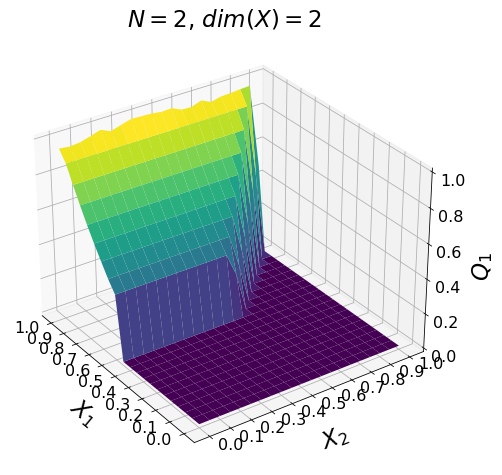
\includegraphics[width=0.6\textwidth]{images/symmetric_independent_unif_01_Q1.png}
        \end{center}
        
        \vspace{1mm}
        \raggedright{\small {\sc Figure \refstepcounter{fig}\thefig\label{fig:belloni_n2_q1}:} The interim allocation $Q_1$ for the first quality grade in the setting of symmetric, independent uniform setting of \autocite{pavlov2011optimal} when $X \sim U[0,1]^2$. Notice, for example, the allocation is monotonic in values of $X_1$ and that the reserve price $p \in [.5, .6)$.}
    \end{figure}

    \item Based on the description of the exclusive buyer mechanism in Section \ref{subsec_ebm}, check if it matches the interim allocations yielded by the approximation algorithm. In Figure (\ref{fig:belloni_n2_q1}), the interim allocation can approximated by the interim allocation for the exclusive buyer mechanism (above): 
    \begin{equation}
        Q_1(x;p) = \mathbbm{1}\{ \beta_1 > \beta_2 \text{ and } \beta_1 \geq 0 \}F^{N-1}(x_1, \min\{\overline{x}_2, r_2 + \beta_1\})
    \end{equation}
    \noindent Examination of the interim allocations of mechanisms yielded by the approximation algorithms is the basis for hypotheses concerning the optimal mechanisms.
\end{enumerate}

\noindent By considering a wide enough range of cases and leveraging results from existing research in multidimensional mechanism design, we can develop some economic intuitions about the qualitative features of optimal mechanisms in a comparatively simpler multidimensional setting without worrying about the problem of bundling in the setting of multiple bidders \textit{and} multiple goods. Since this approach is broadly susceptible to problems of discretization when approximating the optimal mechanism as well as precision issues with numerical computing, conclusions are, at best, a promising guide to developing further theoretical results. Thus, results are best interpreted as conjectures concerning the character of optimal mechanisms in multidimensional settings.




\subsection{Conjectures}\label{subsec_conj}

The principal conjecture investigated in this thesis chapter concerns the optimality of the exclusive buyer mechanism in the multidimensional setting of a single good with multiple quality levels:

\begin{conjecture}[Revenue]\label{conj_rev}
The revenue of the exclusive buyer mechanism well-approximates the revenue of the optimal mechanism.
\end{conjecture}

\noindent By measuring the discrepancy between revenue from the exclusive buyer mechanism and that returned by the approximation algorithm it is possible to confirm or reject this conjecture. 

It is also important to explore the interim allocations yielded by the approximation algorithm and compare them to those of the exclusive buyer mechanism. There should be visual confirmation that the optimal mechanism yielded by the algorithm is qualitatively similar to the exclusive buyer mechanism:

\begin{conjecture}[Allocations]\label{conj_alloc}
The allocation of the exclusive buyer mechanism well-approximates the allocation of the optimal mechanism yielded by the approximation algorithm.
\end{conjecture}

\noindent Note, if conjecture \ref{conj_alloc} holds, it automatically implies \ref{conj_rev}, since the allocations include the reserve price from which the revenue is calculated. However, since it is possible that the exclusive buyer mechanism approximates the revenue of the optimal mechanism but fails to share qualitative features of its allocation, it is helpful to distinguish between both conjectures.

Additionally, a surprising feature of some optimal mechanisms in the setting of a single good with multiple quality levels noted by several economists is that the set of types excluded by the allocation---the \textit{exclusion region}---in equilibrium sometimes has measure zero (e.g., \cite{thirumulanathan2019, belloni2010multidimensional}). This surprising finding stands in opposition to the result of \autocite{armstrong1996multiproduct}, where it was shown that in the case of a multiproduct monopolist that it is always optimal to exclude a positive measure of buyers. Thus, we explore under what circumstances the exclusion region is measure zero. Specifically, we conjecture:

\begin{conjecture}[Measure Zero Exclusion Region]\label{conj_excl_zero}
There exist multidimensional settings where a single good with multiple quality levels is sold to multiple bidders with a measure zero exclusion region.
\end{conjecture}

Finally, we conjecture that the exclusion region does not change with the number of bidders.

\begin{conjecture}[Same Exclusion Region for all $N$]\label{conj_excl_n}
The exclusion region of the optimal mechanism in the multidimensional setting of a single good with multiple quality levels remains the same for $N=1,2,3,\dots$ bidders. 
\end{conjecture}









\subsection{Simulations}\label{subsec_sim}

In what follows we explore conjectures \ref{conj_rev}, \ref{conj_alloc}, \ref{conj_excl_n} in the following contexts:

\begin{enumerate}
    \item The \textbf{symmetric, independent, and uniform setting}, where buyers' valuations are independent across quality grades, uniformly and symmetrically distributed. I analyze the case where two bidders have identical valuations for a good with two quality grades, where each valuation is assumed to be distributed $X_1,X_2 \sim U[0,1]$. Additionally, I analyze the case where $X_1,X_2 \sim U[2,3]$ since, in contrast to the previous setting, it is known that in these settings the optimal mechanism involves randomization when $N=1$. Analytic results in the single buyer case when $X \sim U[c,c+1]^2$ are known \autocite{pavlov2011optimal} and serve as a benchmark.

    \item The \textbf{symmetric, independent, and non-uniform setting}. Here, it is desirable to see if the conclusions reached in the first setting extend to non-uniform distributions. In particular, we consider the case of the $Beta(\alpha,\beta)$ distribution (where $\alpha=1,\beta=2$), which was explored in \autocite{daskalakis2017strong} in the context of multiple-goods.  

    \item The \textbf{symmetric, correlated setting}. It is unknown how arbitrary correlations between a buyer's dimensions of value affect the revenue-maximization problem faced by the auction designer in multidimensional settings. This setting aims to shed light on this problem by considering buyers with valuations drawn from $X_1 = X_2 = [0,1]$ where the distribution of valuations is $f(x_1,x_2) = x_1 + x_2$.

    \item The \textbf{asymmetric, independent, and uniform setting}. No analytic results are known in this similar setting; however, a very provisional analysis of the optimality of the exclusive buyer mechanism in this setting can be found in \autocite{belloni2010multidimensional}, where $X_1 \sim U[6,8], X_2 \sim U[9,11]$ with costs $c_1 = .9, c_2 = 5$. I replicate their analyses and extend their results in the context of the three conjectures proposed above.

    \item The \textbf{asymmetric, independent, and non-uniform setting}, a direct extension of the above setting where the valuations for each quality level of the good are drawn from two different truncated normal distributions. In particular, I consider the case where $X_1 \sim truncnorm(\mu=2.3, \sigma=1, \underline{x}_1=2, \overline{x}_1=3)$ and $X_2 \sim truncnorm(\mu=2.8, \sigma=.2, \underline{x}_2=2, \overline{x}_2=3)$.
\end{enumerate}




\subsubsection{Symmetric, independent, and uniform}

Analytic results in the case of a single buyer exist in the symmetric, independent, and uniform setting considered here. \autocite{pavlov2011optimal} studied the case of two substitute goods\footnote{Note that when there is a single buyer an equivalent interpretation of the setting with one good and multiple quality levels is that there are multiple goods but the buyer has unit demand.} independently and uniformly distributed on $U[c,c+1]^2$. In the specific case of a single buyer with valuations distributed according to $X \sim U[0,1]^2$ with zero costs, it is known that the optimal mechanism is deterministic and involves setting reserve price $p^* =\frac{1}{\sqrt{3}}$ for both goods (since the valuations are symmetric). Thus, the optimal allocation is given in Figure \ref{fig:pavlov_alloc} and the auctioneer's revenue is simply $p^*( 1 - p^{*2} ) = 0.3849...$.
 
\begin{figure}[H]
    \begin{center}
    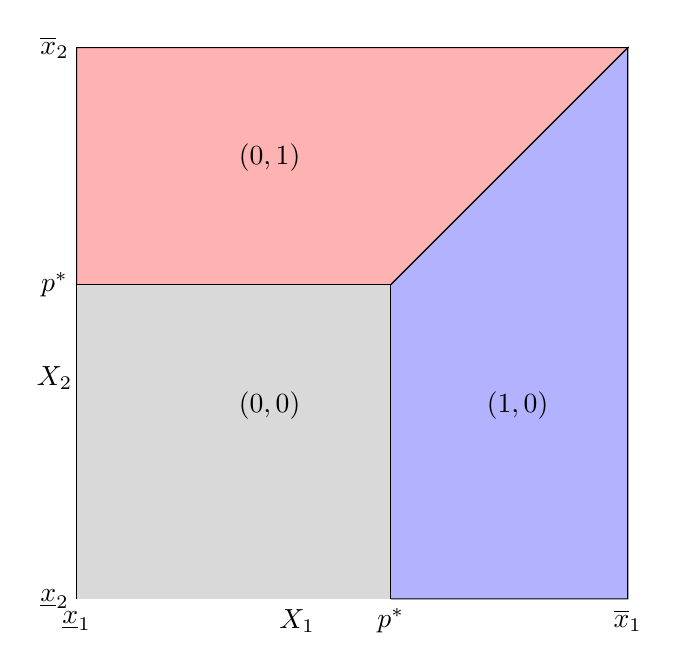
\begin{tikzpicture}[scale=.7]

    % square
    \draw (0,0) rectangle (10,10);

    % lines
    \draw (5.7,0) -- (5.7,5.7);
    \draw (0,5.7) -- (5.7,5.7);
    \draw (5.7,5.7) -- (10,10);

    % fill
    \draw[fill=red!30] (0,5.7) -- (0,10) -- (10,10) -- (5.7,5.7);
    \draw[fill=blue!30] (5.7,0) -- (10,0) -- (10,10) -- (5.7,5.7);
    \draw[fill=gray!30] (0,0) -- (0,5.7) -- (5.7,5.7) -- (5.7,0);

    % axis labels
    \node at (0,-.4) {$\underline{x}_1$};
    \node at (10,-.4) {$\overline{x}_1$};
    \node at (4,-.4) {$X_1$};
    \node at (5.7,-.4) {$p^*$};
    \node at (-.4,0) {$\underline{x}_2$};
    \node at (-.4,10) {$\overline{x}_2$};
    \node at (-.4,4) {$X_2$};
    \node at (-.4,5.7) {$p^*$};

    % region labels and lines
    \node at (3.5,3.5) {$(0,0)$};
    \node at (8,3.5) {$(1,0)$};
    \node at (3.5,8) {$(0,1)$};
    \end{tikzpicture}
    \end{center}
  
    \vspace{1mm}
    \raggedright{\small {\sc Figure \refstepcounter{fig}\thefig\label{fig:pavlov_alloc}:} The optimal allocation of a single good with two quality symmetric levels to a single buyer with valuations $X \sim U[0,1]^2$ \autocite{pavlov2011optimal}. The area denoted $(0,0)$ is the `exclusion region', where the good is not allocated. Note, in the setting of \autocite{pavlov2011optimal}, $p^*=\sqrt{1/3}$.}
\end{figure}

In the case where there is more than one bidder we need to rely on the approximation algorithm to study the qualitative features of the optimal mechanism. First, we can confirm the approximation algorithm yields similar revenue to that calculated by the appropriate exclusive buyer mechanism in this setting. These results are presented in Table \ref{table:pavlov_n2_revenue}.

\begin{center}
    \begin{tabular}{ |c|c|c| } 
    \hline
    Result Type & $T$ & Revenue \\
    \hline
    \hline
    approximation & 5 & 0.66094... \\ 
    approximation & 10 & 0.625929... \\ 
    approximation & 15 & 0.612877... \\ 
    approximation & 20 & 0.606033... \\ 
    exclusive buyer mechanism & 50 & 0.589052... \\
    \hline
    \end{tabular}

    \vspace{1mm}
    \raggedright{\small {\sc Table \refstepcounter{fig}\thefig\label{table:pavlov_n2_revenue}:} comparison of revenue generated by approximation algorithm with that of the exclusive buyer mechanism. $T$ represents the number of intervals used to discretize each dimension of the buyers' valuations.}
\end{center}

\noindent Note that the revenue generated by the exclusive buyer mechanism was computed using the \textit{ex-post} description of the auction. Additionally, the exclusive buyer mechanism's revenue was computed by numerical integration on a finder discretization grid as that used by the approximation algorithm for increased precision. The trend for different $T$ implies that the approximation algorithm is converging to the result provided by the exclusive buyer mechanism. This supports Conjecture \ref{conj_rev}. 

Using the \textit{interim} allocation of the exclusive buyer mechanism described in section (\ref{subsec_ebm}), we can plot the allocations against those returned by the approximation algorithm. These are presented side-by-side in Figure \ref{fig:pavlov_n2_alloc}.

\begin{figure}[H]
    \begin{center}
    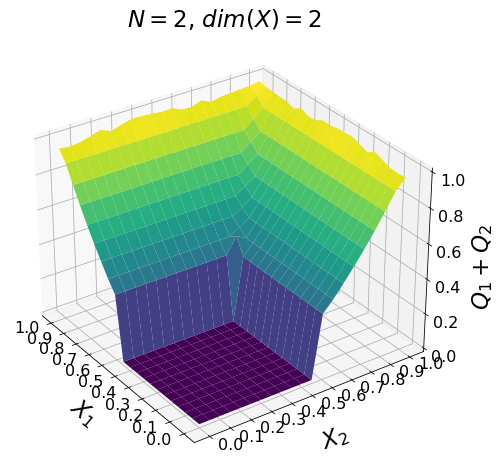
\includegraphics[width=0.45\textwidth]{images/symmetric_independent_unif_01.png}
    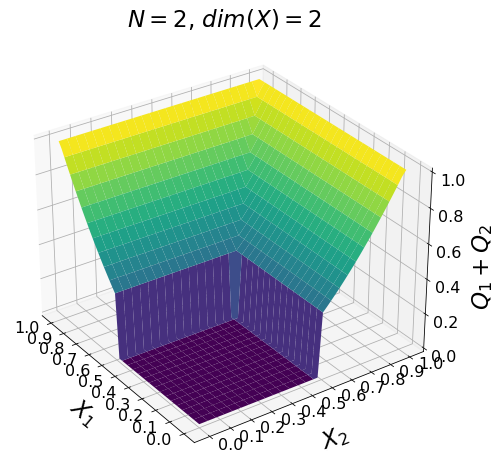
\includegraphics[width=0.44\textwidth]{images/symmetric_independent_unif_01_ebm.png}
    \end{center}
    
    \vspace{1mm}
    \raggedright{\small {\sc Figure \refstepcounter{fig}\thefig\label{fig:pavlov_n2_alloc}:} The allocations produced by the approximation algorithm (left) and exclusive buyer mechanism (right).} 
\end{figure}

\noindent Conjecture \ref{conj_alloc} requires qualitatively evaluating the allocations returned from the approximation algorithm and those calculated from the exclusive buyer mechanism, without an obvious means to conclusively determine whether the conjecture is supported. However, the results in Figure \ref{fig:pavlov_n2_alloc} imply that exclusive buyer mechanism captures the behavior of the (approximately) optimal mechanism. Thus, these results offer support for Conjecture \ref{conj_alloc}.

Notice that the exclusion region in Figure \ref{fig:pavlov_n2_alloc} is similar to that discovered in \autocite{pavlov2011optimal}. This is evidence against Conjecture \ref{conj_excl_zero} concerning the existence of measure zero exclusion regions. The price $p^* = \frac{1}{\sqrt{3}} = 0.577...$ that maximizes revenue in the case when $N=1$ is consistent with the exclusion region defined by $p^* = 0.6$ returned by the approximation algorithm for the case of $N=2$. (Note that when $[0,1]$ is discretized into 20 intervals, the price is $p \in \{\dots, .5, .55, .6, \dots\}$ so the choice by the algorithm reflects its approximate optimality). Indeed, when $T=20$, the approximation algorithm yields the same exclusion region for all of $N=1,2,3$. This supports Conjecture \ref{conj_excl_n}.

% \begin{figure}[H]
%     \begin{center}
%     \begin{tikzpicture}[scale=.7]
%     % square
%     \draw (0,0) rectangle (10,10);

%     % lines
%     \draw (5.77,0) -- (5.77,5.77);
%     \draw (0,5.77) -- (5.77,5.77);
%     \draw (5.77,5.77) -- (10,10);

%     % fill
%     \draw[fill=gray!30] (0,0) -- (0,5.77) -- (5.77,5.77) -- (5.77,0);

%     % axis labels
%     \node at (0,-.4) {$\underline{x}_1$};
%     \node at (10,-.4) {$\overline{x}_1$};
%     \node at (4,-.4) {$X_1$};
%     \node at (5.77,-.4) {$p^*$};
%     \node at (-.4,0) {$\underline{x}_2$};
%     \node at (-.4,10) {$\overline{x}_2$};
%     \node at (-.4,4) {$X_2$};
%     \node at (-.4,5.77) {$p^*$};

%     % region labels and lines
%     \node at (3.5,3.5) {$(0,0)$};

%     \end{tikzpicture}
%     \end{center}
  
%     \vspace{1mm}
%     \raggedright{\small {\sc Figure \refstepcounter{fig}\thefig\label{fig:pavlov_all_n_excl}:} The exclusion region produced by the approximation algorithm when $T=20$ for each of $N=1,2,3$. As noted above, due to the discretization $T=20$, $p^* = 0.6$.}
% \end{figure}

Furthermore, it is helpful to investigate the behavior of the approximation algorithm when $X \sim U[2,3]^2$, since we know from Pavlov \autocite*{pavlov2011optimal} that the optimal mechanism is stochastic. This is particularly important in the context of Conjecture \ref{conj_excl_n} since it implies that the exclusive buyer mechanism will not be optimal in this case.

Again, first we confirm the approximation algorithm yields similar revenue to that calculated by the appropriate exclusive buyer mechanism in this setting. These results are presented in Table \ref{table:pavlov_23_n2_revenue}.

\begin{center}
    \begin{tabular}{ |c|c|c| } 
    \hline
    Result Type & $T$ & Revenue \\
    \hline
    \hline
    approximation & 5 & 2.622409... \\ 
    approximation & 10 & 2.58287... \\ 
    approximation & 15 & 2.58287... \\ 
    approximation & 20 & 2.562314... \\ 
    exclusive buyer mechanism & 50 & 2.534499... \\
    \hline
    \end{tabular}

    \vspace{1mm}
    \raggedright{\small {\sc Table \refstepcounter{fig}\thefig\label{table:pavlov_23_n2_revenue}:} comparison of revenue generated by approximation algorithm with that of the exclusive buyer mechanism. Since the mechanism yielded by the approximation algorithm included randomization and, therefore, the menu of contract points included more than a single reserve price, the choice of reserve price for exclusive buyer mechanism was $r=2.15$.}
\end{center}

\noindent Here, the exclusive buyer mechanism yields a revenue similar to that of the optimal mechanism. The difference between the revenues is approximately 1\%, despite the stochastic optimal mechanism. Furthermore, there is a clear indication that as $T$ increases, the approximation algorithm converges to the revenue yielded by the exclusive buyer mechanism. This supports Conjecture \ref{conj_rev}.

We can plot the allocations of the optimal mechanism generated by the approximation algorithm with those of the exclusive buyer mechanism to assess our next conjecture. These are presented side-by-side in Figure \ref{fig:pavlov_n2_23_alloc}.

\begin{figure}[H]
    \begin{center}
    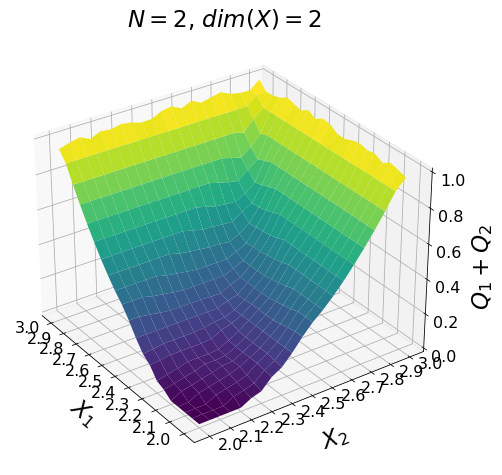
\includegraphics[width=0.45\textwidth]{images/symmetric_independent_unif_23.png}
    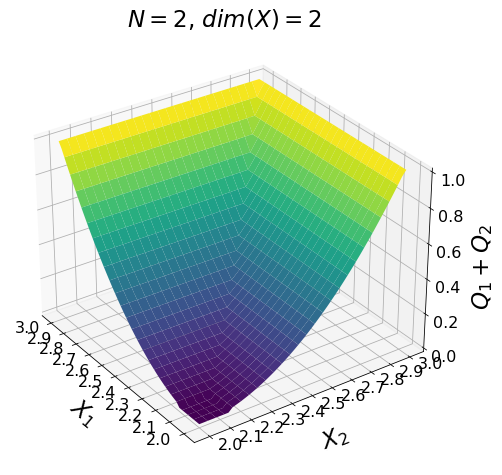
\includegraphics[width=0.44\textwidth]{images/symmetric_independent_unif_23_ebm.png}
    \end{center}
    
    \vspace{1mm}
    \raggedright{\small {\sc Figure \refstepcounter{fig}\thefig\label{fig:pavlov_n2_23_alloc}:} The allocations produced by the approximation algorithm (left) and exclusive buyer mechanism (right).} 
\end{figure}

\noindent Although the shape of the allocations is similar in the region where $Q_1(x) + Q_2(x) > 0$, the exclusion region yielded by the optimal mechanism is triangular, indicating that the optimal mechanism includes randomization. In contrast, the exclusive buyer mechanism is a deterministic mechanism and has a rectangular exclusion region. Thus, this setting does not support Conjecture \ref{conj_alloc}.

Again, the exclusion region in Figure \ref{fig:pavlov_n2_23_alloc} is similar to that discovered in \autocite{pavlov2011optimal}. This is notable because when $X \sim [c,c+1]^2$ there was randomization in the single bidder case. This is both evidence against Conjecture \ref{conj_excl_zero} concerning the existence of measure zero exclusion regions and evidence for Conjecture \ref{conj_excl_n}. Indeed, when $T=20$, the approximation algorithm yields the same exclusion region for all of $N=1,2,3$.





\subsubsection{Symmetric, independent, and non-uniform setting}

I examine the four conjectures in the context of a symmetric, independent, and non-uniform setting. Following the multi-unit example in \autocite{daskalakis2017strong}, I consider the case where $X_1,X_2 \sim Beta(\alpha,\beta)$ where $\alpha=1,\beta=2$. To the best of my knowledge, no prior work on analytic solutions to the optimal auction design problem exists in this setting. Therefore, we proceed by running the optimization algorithm and comparing the output of the algorithm to that provided by the exclusive buyer mechanism described above.

First, we compare the revenue generated by the approximation algorithm and the exclusive buyer mechanism. The results are presented in Table \ref{table:symm_beta_revenue}. Again, note the revenue from the exclusive buyer mechanism was calculated using \textit{ex-post} allocations from a second-price auction. Although the revenue generated from the optimal mechanism is larger than the exclusive buyer mechanism ($\sim$4\%), the trend as $T$ increases provides support for Conjecture \ref{conj_rev}.

\begin{center}
    \begin{tabular}{ |c|c|c| } 
    \hline
    Result Type & $T$ & Revenue \\
    \hline
    \hline
    approximation & 5 & 0.448709... \\ 
    approximation & 10 & 0.418815... \\ 
    approximation & 15 & 0.406948... \\ 
    approximation & 20 & 0.400615... \\ 
    exclusive buyer mechanism & 50 & 0.385045... \\
    \hline
    \end{tabular}

    \vspace{1mm}
    \raggedright{\small {\sc Table \refstepcounter{fig}\thefig\label{table:symm_beta_revenue}:} comparison of revenue generated by the approximation algorithm with that of the exclusive buyer mechanism when $X_1,X_2 \sim Beta(1,2)$.}
\end{center}

Next, we can compare the interim allocations from the approximation algorithm with those from the exclusive buyer mechanism. These are displayed graphically in Figure \ref{fig:beta12_alloc}. There is a clear similarity between both allocations, supporting Conjecture \ref{conj_alloc}.

\begin{figure}[H]
    \begin{center}
    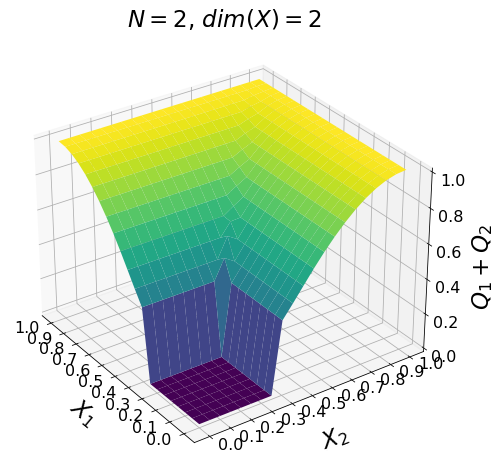
\includegraphics[width=0.45\textwidth]{images/symmetric_independent_beta.png}
    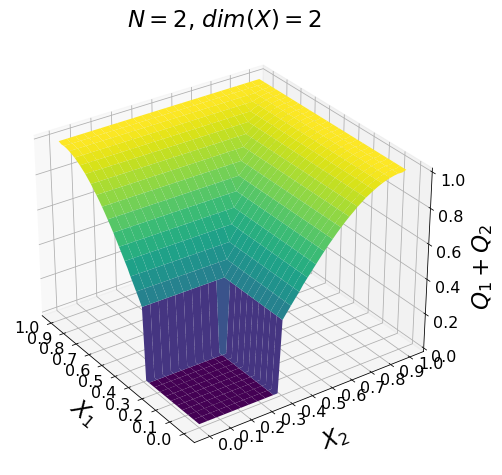
\includegraphics[width=0.44\textwidth]{images/symmetric_independent_beta_ebm.png}
    \end{center}
    
    \vspace{1mm}
    \raggedright{\small {\sc Figure \refstepcounter{fig}\thefig\label{fig:beta12_alloc}:} The allocations produced by the approximation algorithm (left) and exclusive buyer mechanism (right).} 
\end{figure}


\noindent Note, these allocations offer a lack of support of Conjecture \ref{conj_excl_zero} concerning the existence of measure zero exclusion regions.

Finally, running the approximation algorithm for $N=1,2,3$ confirms Conjecture \ref{conj_excl_n}. The exclusion region is the same for all $N$ tested: the value of $p^*=0.4$. (Recall, discretization of the grid into $T=20$ intervals per quality level requires that $p^* \in \{\dots, 0.35, 0.4, 0.45, \dots\}$).  

% \begin{figure}[H]
%     \begin{center}
%     \begin{tikzpicture}[scale=.7]
%     % square
%     \draw (0,0) rectangle (10,10);

%     % lines
%     \draw (4,0) -- (4,4);
%     \draw (0,4) -- (4,4);

%     % fill
%     \draw[fill=gray!30] (0,0) -- (0,4) -- (4,4) -- (4,0);

%     % axis labels
%     \node at (0,-.4) {$\underline{x}_1$};
%     \node at (10,-.4) {$\overline{x}_1$};
%     \node at (4,-.4) {$p^*$};
%     \node at (6,-.4) {$X_1$};
%     \node at (-.4,0) {$\underline{x}_2$};
%     \node at (-.4,10) {$\overline{x}_2$};
%     \node at (-.4,4) {$p^*$};
%     \node at (-.4,6) {$X_2$};

%     % region labels and lines
%     \node at (2,2) {$(0,0)$};
%     \end{tikzpicture}
%     \end{center}
  
%     \vspace{1mm}
%     \raggedright{\small {\sc Figure \refstepcounter{fig}\thefig\label{fig:beta12_all_n_excl}:} The exclusion region produced by the approximation algorithm when $T=20$ for each of $N=1,2,3$. Note, in this setting, $p^*=0.4$.}
% \end{figure}

Thus, in conclusion, all conjectures are supported in the setting of symmetric, independent, and non-uniform distributions except for Conjecture \ref{conj_excl_zero} concerning the existence of a measure zero exclusion region.







\subsubsection{Symmetric, correlated setting}

In this setting, I allow for the valuations $X_1$ and $X_2$ to be correlated. Here, $X_1 = X_2 = [0,1]$, where $X \sim F$ and $f(x_1,x_2) = x_1+x_2$. This extension of the previous settings on the unit square facilitates a deeper understanding of correlated valuations in a familiar setting. As above, I proceed by running the approximation algorithm and comparing the results with those from the exclusive buyer mechanism.

With regard to revenue, we can see in Table \ref{table:symm_correlated_revenue} that the algorithm's revenue is, again, well-approximated by the exclusive buyer mechanism ($\sim$3\%). The trend as $T$ increases is similar to the other settings: the revenue generated by the approximation algorithm converges to that yielded by the exclusive buyer mechanism. This supports Conjecture \ref{conj_rev}.

\begin{center}
    \begin{tabular}{ |c|c|c| } 
    \hline
    Result Type & $T$ & Revenue \\
    \hline
    \hline
    approximation & 5 & 0.75159... \\ 
    approximation & 10 & 0.718683... \\ 
    approximation & 15 & 0.705905... \\ 
    approximation & 20 & 0.698962... \\ 
    exclusive buyer mechanism & 50 & 0.676192... \\
    \hline
    \end{tabular}

    \vspace{1mm}
    \raggedright{\small {\sc Table \refstepcounter{fig}\thefig\label{table:symm_correlated_revenue}:} comparison of revenue generated by the approximation algorithm with that of the exclusive buyer mechanism when $f(x_1,x_2) = x_1 + x_2$.}
\end{center}

The allocations are also similar. The interim allocations from the approximation algorithm and the exclusive buyer mechanism are presented in Figure \ref{fig:symmetric_correlated_alloc}. This supports Conjecture \ref{conj_alloc} concerning the qualitative similarity of the optimal mechanism yielded by the approximation algorithm and that of the exclusive buyer mechanism.

\begin{figure}[H]
    \begin{center}
    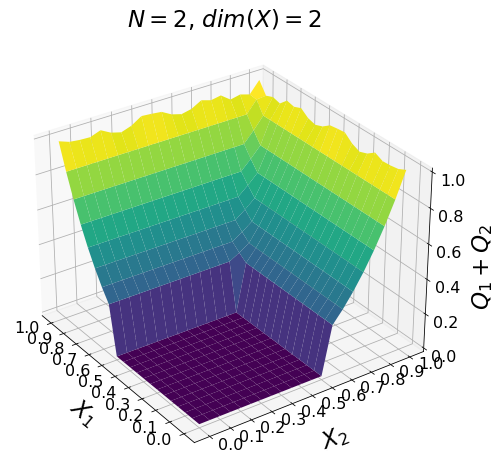
\includegraphics[width=0.45\textwidth]{images/symmetric_correlated_unif.png}
    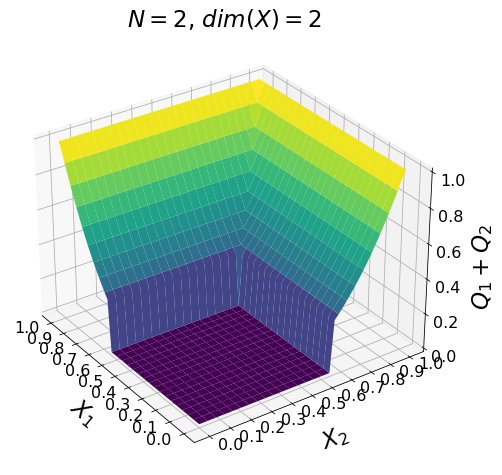
\includegraphics[width=0.44\textwidth]{images/symmetric_correlated_unif_ebm.png}
    \end{center}
    
    \vspace{1mm}
    \raggedright{\small {\sc Figure \refstepcounter{fig}\thefig\label{fig:symmetric_correlated_alloc}:} The allocations produced by the approximation algorithm (left) and the exclusive buyer mechanism (right).} 
\end{figure}

\noindent Again, note the presence of an exclusion region undermines support for Conjecture \ref{conj_excl_zero} concerning the existence of settings without an exclusion region.

Finally, the exclusion regions in the symmetric, correlated, uniform setting where $X_1 = X_2 = [0,1]$ and $f(x_1,x_2) = x_1 + x_2$ are the same for all $N=1,2,3$. Note, the reserve price is $p^* = .65$ in this setting. This supports Conjecture \ref{conj_excl_n}.

% \begin{figure}[H]
%     \begin{center}
%     \begin{tikzpicture}[scale=.7]
%     % square
%     \draw (0,0) rectangle (10,10);

%     % lines
%     \draw (6.5,0) -- (6.5,6.5);
%     \draw (0,6.5) -- (6.5,6.5);

%     % fill
%     \draw[fill=gray!30] (0,0) -- (0,6.5) -- (6.5,6.5) -- (6.5,0);

%     % axis labels
%     \node at (0,-.4) {$\underline{x}_1$};
%     \node at (10,-.4) {$\overline{x}_1$};
%     \node at (6.5,-.4) {$p^*$};
%     \node at (4,-.4) {$X_1$};
%     \node at (-.4,0) {$\underline{x}_2$};
%     \node at (-.4,10) {$\overline{x}_2$};
%     \node at (-.4,6.5) {$p^*$};
%     \node at (-.4,4) {$X_2$};

%     % region labels and lines
%     \node at (3.5,3.5) {$(0,0)$};
%     \end{tikzpicture}
%     \end{center}
  
%     \vspace{1mm}
%     \raggedright{\small {\sc Figure \refstepcounter{fig}\thefig\label{fig:symm_correlated_all_n_excl}:} The exclusion region produced by the approximation algorithm when $T=20$ for each of $N=1,2,3$. Note, in this setting, $p^*=.65$.}
% \end{figure}

As in the previous setting, all conjectures except for Conjecture \ref{conj_excl_zero} concerning the existence of a measure zero exclusion region are supported.








\subsubsection{Asymmetric, independent, and uniform setting}

In this setting, we consider the case where $X_1 \sim U[6,8]$ and $X_2 \sim U[9,11]$ as considered in \autocite{belloni2010multidimensional}, who first studied the optimality of the exclusive buyer mechanism in multidimensional settings. Additionally, the costs associated with selling the first quality grade of the good are $c_1 = .9$ and the second quality grade are $c_2 = 5$. Since prior computational work exists assessing the optimality of the exclusive buyer mechanism, where possible, I can compare my findings here with those in \autocite{belloni2010multidimensional}. 

The revenue yielded by the approximation algorithm is similar to that of the exclusive buyer mechanism. The data are displayed in Table \ref{table:asymm_belloni}. These revenue numbers are consistent with those in \autocite[Table 3]{belloni2010multidimensional}, supporting Conjecture \ref{conj_rev}, namely, that the revenue of the optimal mechanism is well-approximated by the exclusive buyer mechanism.

\begin{center}
    \begin{tabular}{ |c|c|c| } 
    \hline
    Result Type & $T$ & Revenue \\
    \hline
    \hline
    approximation & 5 & 6.02496... \\ 
    approximation & 10 & 5.941549... \\ 
    approximation & 15 & 5.91222... \\ 
    approximation & 20 & 5.893113... \\ 
    exclusive buyer mechanism & 50 & 5.805032... \\
    \hline
    \end{tabular}

    \vspace{1mm}
    \raggedright{\small {\sc Table \refstepcounter{fig}\thefig\label{table:asymm_belloni}:} comparison of revenue generated by the approximation algorithm with that of the exclusive buyer mechanism in the setting of \autocite{belloni2010multidimensional}.}
\end{center}

With regard to the allocations, we can see a clear disparity between the interim allocations produced by the approximation algorithm and those of the exclusive buyer mechanism. The exclusive buyer mechanism's interim allocation for $Q_1(x) + Q_2(x)$ is much lower for large values of $X_2$ than that of the approximation algorithm. The allocations are presented in Figure \ref{fig:belloni_alloc}.

\begin{figure}[H]
    \begin{center}
    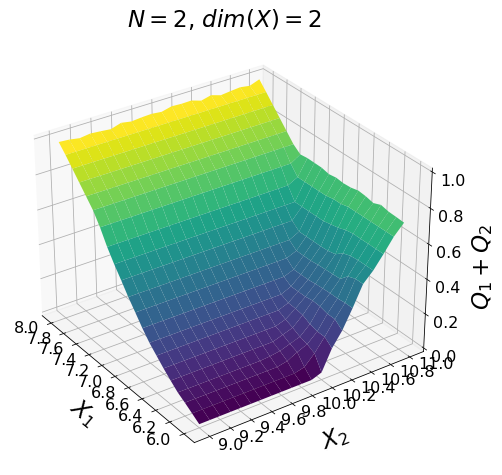
\includegraphics[width=0.45\textwidth]{images/asymmetric_independent_belloni.png}
    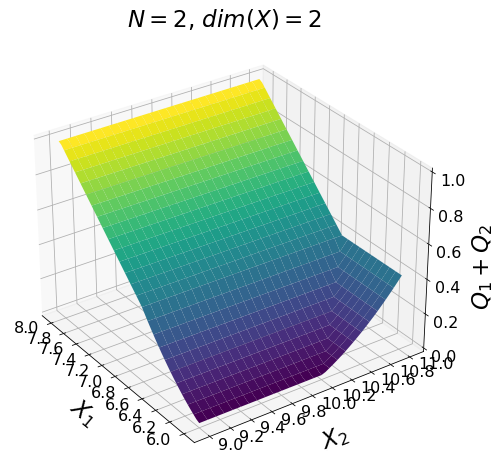
\includegraphics[width=0.44\textwidth]{images/asymmetric_independent_belloni_ebm.png}
    \end{center}
    
    \vspace{1mm}
    \raggedright{\small {\sc Figure \refstepcounter{fig}\thefig\label{fig:belloni_alloc}:} The allocations produced by the approximation algorithm (left) and the exclusive buyer mechanism (right).} 
\end{figure}

\noindent This surprising feature of the exclusive buyer mechanism's interim allocation suggests that Conjecture \ref{conj_alloc} is \textit{not} supported in the asymmetric, independent, and uniform setting. Here, although the optimal revenue is well approximated by the exclusive buyer mechanism, the qualitative features of the optimal mechanism are sufficiently different from those conjectured by the exclusive buyer mechanism. We will explore this result in more detail in the discussion section (\ref{sec_discuss}) below.

Notice, however, in this setting Conjecture \ref{conj_excl_zero} is supported. This is visible in Figure \ref{fig:belloni_alloc_alln} below. This was also noted in the simulations \autocite{belloni2010multidimensional}, suggesting it is robust to computational or approximation error. Additionally, Conjecture \ref{conj_excl_n} is supported for all $N=1,2,3$; however, it is important to note a number of surprising features of the optimal mechanism yielded by the approximation algorithm in this setting. Firstly, although the exclusion region is the same for all $N$, the \textit{allocation} itself varies with the number of buyers. Secondly, there is evidence of randomization in the optimal mechanism yielded by the approximation algorithm. 

\begin{figure}[H]
    \begin{center}
    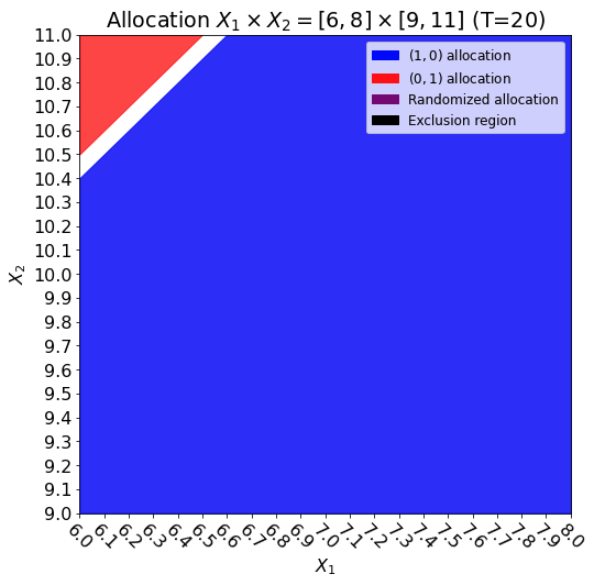
\includegraphics[width=0.45\textwidth]{images/belloni_alloc_n1.png}
    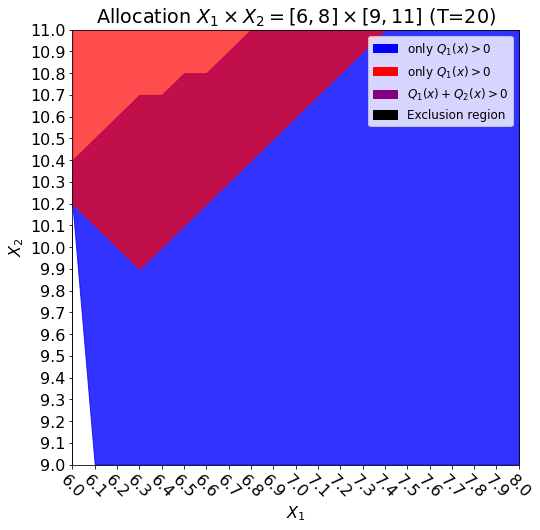
\includegraphics[width=0.44\textwidth]{images/belloni_alloc_n2.png}
    \end{center}
    
    \vspace{1mm}
    \raggedright{\small {\sc Figure \refstepcounter{fig}\thefig\label{fig:belloni_alloc_alln}:} Graphs showing where the allocations for the first ($Q_1$) and second ($Q_2$) quality level of the good are non-zero for the optimal mechanism yielded by the approximation algorithm for $N=1$ (left) and $N=2$ (right).} 
\end{figure}

Thus, in the symmetric correlated setting, although Conjectures \ref{conj_rev}, \ref{conj_excl_zero}, \ref{conj_excl_n} are supported, Conjecture \ref{conj_alloc} is not. The complexities of this result will be further explored below.







\subsubsection{Asymmetric, independent, and non-uniform setting}

I extend the investigation of asymmetric settings by considering the cases where buyers' valuations are distributed according to two different distributions. In particular, I consider the case where the valuations are drawn from $X_1 = X_2 = [2,3]$ and the distribution of valuations is asymmetric, where $X_1 \sim truncnorm(\mu=2.3, \sigma=1)$ and $X_2 \sim truncnorm(\mu=2.8, \sigma=.2)$. Note, in contrast to the previous asymmetric setting considered above, in this setting the sets from which the valuations are drawn are equal (i.e., $X_1 = X_2$) but the distributions are not (i.e., $f_1(x) \neq f_2(x)$). Again, no prior analytic results exist in this setting and therefore I proceed by running the approximation algorithm for the optimal auction and comparing the result to that of the exclusive buyer mechanism.

First, I compare the revenue generated by the approximation algorithm and the exclusive buyer mechanism. This is presented in Table \ref{table:asymm_truncnorm_revenue}. The similarity of the revenues generated by the approximation algorithm and the exclusive buyer mechanism lends support to Conjecture \ref{conj_rev}.

\begin{center}
    \begin{tabular}{ |c|c|c| } 
    \hline
    Result Type & $T$ & Revenue \\
    \hline
    \hline
    approximation & 5 & 2.779996... \\ 
    approximation & 10 & 2.749451... \\ 
    approximation & 15 & 2.736171... \\ 
    approximation & 20 & 2.729342... \\ 
    exclusive buyer mechanism & 50 & 2.57921... \\
    \hline
    \end{tabular}

    \vspace{1mm}
    \raggedright{\small {\sc Table \refstepcounter{fig}\thefig\label{table:asymm_truncnorm_revenue}:} comparison of revenue generated by the approximation algorithm with that of the exclusive buyer mechanism when $X_1 \sim truncnorm(\mu=2.3, \sigma=1, \underline{x}_1=2, \overline{x}_1=3)$ and $X_2 \sim truncnorm(\mu=2.8, \sigma=.2, \underline{x}_2=2, \overline{x}_2=3)$.}
\end{center}

When we compare the interim allocations generated by the approximation algorithm to those of the exclusive buyer mechanism in Figure \ref{fig:truncnorm_alloc}, we can qualitatively see that the allocations are similar. This supports Conjecture \ref{conj_alloc}.

\begin{figure}[H]
    \begin{center}
    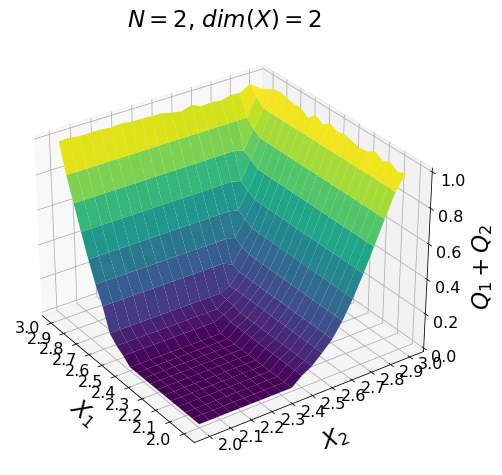
\includegraphics[width=0.45\textwidth]{images/asymmetric_independent_truncnorm.png}
    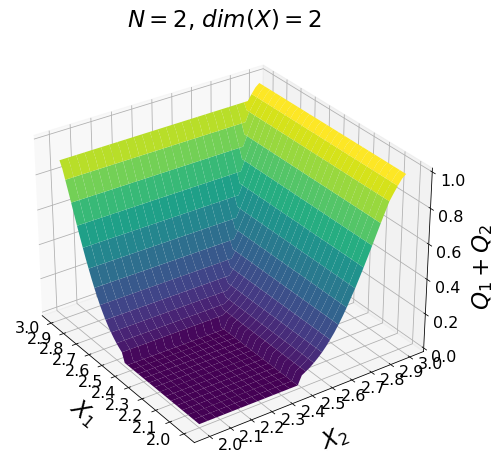
\includegraphics[width=0.44\textwidth]{images/asymmetric_independent_truncnorm_ebm.png}
    \end{center}
    
    \vspace{1mm}
    \raggedright{\small {\sc Figure \refstepcounter{fig}\thefig\label{fig:truncnorm_alloc}:} The allocations produced by the approximation algorithm (left) and exclusive buyer mechanism (right).} 
\end{figure}

\noindent Additionally, note that the existence of an exclusion region in Figure \ref{fig:truncnorm_alloc} above undermines Conjecture \ref{conj_excl_zero}.

Finally, running the approximation algorithm for all $N=1,2,3$ confirms Conjecture \ref{conj_excl_n}. In this asymmetric setting $p_1^* = 2.55$ and $p_2^* = 2.5$ and the exclusion region remains the same for all $N$. 

% \begin{figure}[H]
%     \begin{center}
%     \begin{tikzpicture}[scale=.7]
%     % square
%     \draw (0,0) rectangle (10,10);

%     % lines
%     \draw (5.5,0) -- (5.5,5);
%     \draw (0,5) -- (5.5,5);

%     % fill
%     \draw[fill=gray!30] (0,0) -- (5.5,0) -- (5.5,5) -- (0,5);

%     % axis labels
%     \node at (0,-.4) {$\underline{x}_1$};
%     \node at (10,-.4) {$\overline{x}_1$};
%     \node at (5.5,-.4) {$p_1^*$};
%     \node at (4,-.4) {$X_1$};
%     \node at (-.4,0) {$\underline{x}_2$};
%     \node at (-.4,10) {$\overline{x}_2$};
%     \node at (-.4,5) {$p_2^*$};
%     \node at (-.4,4) {$X_2$};

%     % region labels and lines
%     \node at (2,2) {$(0,0)$};
%     \end{tikzpicture}
%     \end{center}
  
%     \vspace{1mm}
%     \raggedright{\small {\sc Figure \refstepcounter{fig}\thefig\label{fig:truncnorm_all_n_excl}:} The exclusion region produced by the approximation algorithm when $T=20$ for each of $N=1,2,3$. Note, in this setting, $p_1^*=2.55, p_2^*=2.5$.}
% \end{figure}

Thus, in conclusion, all conjectures except for Conjecture \ref{conj_excl_zero} concerning the existence of a measure zero exclusion region are supported in the setting of asymmetric, independent, and non-uniform distributions.




\section{Discussion \& Conclusion}\label{sec_discuss}

Analytic results concerning the qualitative characteristics of optimal auctions in multidimensional settings are scarce. In this chapter, I explored the particular multidimensional setting of a single good with multiple quality levels. In particular, I investigated whether the exclusive buyer mechanism is optimal in this setting. To do this, I developed an approximation algorithm that facilitates the investigation of the optimal mechanism in multidimensional settings and compared the performance of the exclusive buyer mechanism to that of the optimal mechanism yielded by the approximation algorithm across a number of questions. 

I explored four conjectures concerning the optimality of the exclusive buyer mechanism in the multidimensional setting of a single good with multiple quality levels. The rest of this section contains a discussion of how the results presented in Section \ref{subsec_sim} support or undermine these conjectures.

\subsection{Conjecture \ref{conj_rev} (Revenue)}

This conjecture asserted that ``the revenue of the exclusive buyer mechanism well-approximates the revenue of the optimal mechanism''. Across all settings considered above, this conjecture is supported. However, support for this conjecture alone is far from sufficient to demonstrate the optimality of the exclusive buyer mechanism. It is well known that simple (deterministic) mechanisms can approximate optimal (stochastic) mechanisms up to some constant fraction of their revenue. This approximation can often be very close to the revenue yielded by the optimal mechanism. In the case where a single bidder's valuations are uniformly distributed on the unit square $X \sim [c,c+1]^2$, the gain from using a fully optimal mechanism over the best deterministic mechanism is at most 1.2\% \autocite[p11]{pavlov2011optimal}. Though in some settings considered here with $N=2$ bidders, the gain is closer to 3-4\%, the trend as $T$ increases suggests that the final gain from using optimal mechanism over the exclusive buyer mechanism is closer to $\sim$1-2\% in instances where randomization is required for optimality. Furthermore, the results are also consistent with previous simulation studies on the optimality of the exclusive buyer mechanism indicating it well-approximates the revenue generated by the optimal mechanism \autocite{belloni2010multidimensional}. Thus, the results support Conjecture \ref{conj_rev}.

\subsection{Conjecture \ref{conj_alloc} (Allocations)}

Across all settings considered here, the interim allocations of the optimal mechanism yielded by the approximation algorithm share qualitative features with the exclusive buyer mechanism's allocations. However, there are multiple cases where the allocations are noticeably different. Thus, there is mixed support for Conjecture \ref{conj_alloc}, which asserts that ``the allocation of the exclusive buyer mechanism well-approximates the allocation of the optimal mechanism yielded by the approximation algorithm.'' I consider each of these cases in turn.

There is evidence of support for Conjecture \ref{conj_alloc} in the following settings:
\begin{itemize}
    \item Symmetric, independent, and uniform setting ($X \sim U[0,1]^2$)
    \item Symmetric, independent, and non-uniform setting ($X \sim Beta(1,2)^2$)
    \item Symmetric, correlated, and uniform setting ($X \sim F, f(x_1,x_2) = x_1 + x_2$)
    \item Asymmetric, independent, and non-uniform setting ($X_1 \sim truncnorm(\mu=2.3, \sigma=1, \underline{x}_1=2, \overline{x}_1=3)$, $X_2 \sim truncnorm(\mu=2.8, \sigma=.2, \underline{x}_2=2, \overline{x}_2=3)$)
\end{itemize}
\noindent In each of these settings, the reserve prices were consistent and the allocations were qualitatively similar in the region where $Q_1(x) + Q_2(x) > 0$. It is noteworthy that in each of these settings, the optimal mechanism is deterministic. 

There is evidence against Conjecture \ref{conj_alloc} in the symmetric, independent, and uniform setting ($X \sim U[2,3]^2$) and the asymmetric, independent, and uniform setting first investigated by Belloni, Lopomo, and Wang \autocite*{belloni2010multidimensional}. In both these settings there is evidence of randomization in the optimal mechanism, which suggests the deterministic exclusive buyer mechanism is unable to approximate the optimal allocations. In the former case when $X \sim U[2,3]^2$ the exclusion region is not rectangular. In the latter case, the exclusion region has measure zero and, on closer inspection, evidence of randomization can be seen in Figure \ref{fig:belloni_alloc_Q1} where the allocations for each quality grade are shown separately. As can be seen in the graph of $Q_1$ on the left, a ``fold'' in the allocation occurs around the line $x_1 - c_1 = x_2 - c_2$ (recall, $c_1=.9, c_2=5$). In this region, both $Q_1(x) > 0$ and $Q_2(x) > 0$.


\begin{figure}[H]
    \begin{center}
    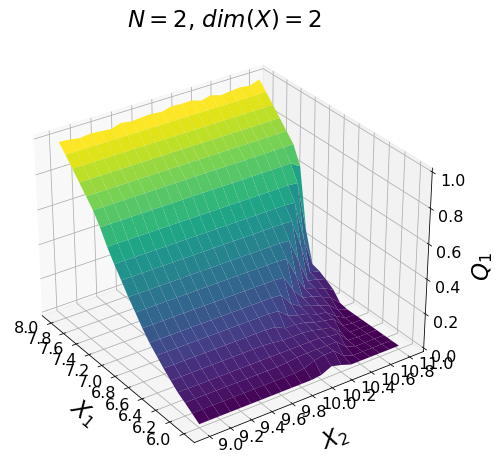
\includegraphics[width=0.45\textwidth]{images/asymmetric_independent_belloni_Q1.png}
    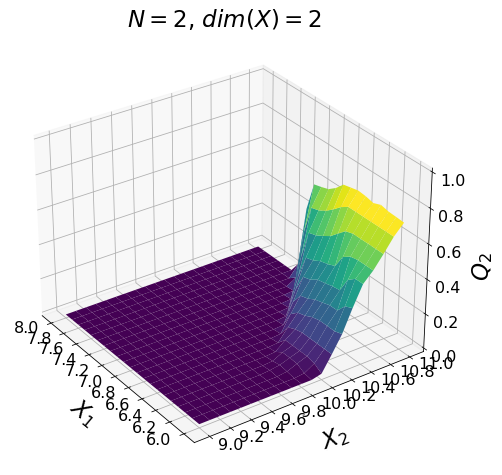
\includegraphics[width=0.45\textwidth]{images/asymmetric_independent_belloni_Q2.png}
    \end{center}
    
    \vspace{1mm}
    \raggedright{\small {\sc Figure \refstepcounter{fig}\thefig\label{fig:belloni_alloc_Q1}:} The allocation $Q_1$ for the first quality level (left) and $Q_2$ for the second quality level (right) of the good produced by the approximation algorithm when $N=2$.} 
\end{figure}

In conclusion, there is mixed support for Conjecture \ref{conj_alloc}. When the optimal mechanism exhibits randomization, the allocations of the deterministic exclusive buyer mechanism do not well-approximate optimal allocations. However, it is possible to construct an \textit{stochastic exclusive buyer mechanism} which includes lotteries. The idea is simple: again, each bidder bids to be the only bidder to choose between quality grades of the object. They can then purchase one of any number of lotteries determined by the seller. This mechanism was not considered in this chapter but future work should address whether it might be optimal in the multidimensional setting of a single good with multiple quality grades.





\subsection{Conjecture \ref{conj_excl_zero} (Measure Zero Exclusion Region)}

Conjecture \ref{conj_excl_zero} concerns the existence of ``multidimensional settings where a single good with multiple quality levels is sold to multiple bidders with a measure zero exclusion region''. Only the asymmetric, independent, and uniform setting initially investigated by Belloni, Lopomo, and Wang \autocite*{belloni2010multidimensional} provides evidence for this conjecture. This finding was also discussed in the work of Thirumulanathan, Sundaresan, and Narahar \autocite*{thirumulanathan2019unitdemand}, who studied the multidimensional setting of a single good with multiple quality levels when bidder valuations are uniformly distributed on an arbitrary rectangle $[a,b] \times [c,d]$. 

This finding stands in contrast to theoretical work in multidimensional mechanism design where it has been shown in the multi-unit case that it is always optimal to exclude a positive measure of bidder types \autocite{armstrong1996multiproduct,rochet1998ironing}. Notice that in the example considered above the typespace $[6,8]\times[9,11]$ violates the assumption of strict convexity. This assumption is essential to establish Armstrong's \autocite*{armstrong1996multiproduct} proof. In the case of Rochet and Choné \autocite*{rochet1998ironing}, they require the cost function to be smooth, which is clearly violated in the setting above.

Figure \ref{fig:belloni_alloc} suggests that for the mechanism yielded by the approximation algorithm, there is an interval $6\times [9,p^*]$ for some $p^*\in [9,11]$ that receives zero utility in equilibrium. The measure of this interval is zero. However, contrary to \autocite[Proposition 1]{armstrong1996multiproduct}, if one increases the price by $\epsilon$, one would exclude a mass of types proportional to $\epsilon$ and not $\epsilon^2$. This intuition suggests why optimal mechanisms might be characterized by measure zero exclusion regions in asymmetric settings. 





\subsection{Conjecture \ref{conj_excl_n} (Same Exclusion Region for all $N$)}

Conjecture \ref{conj_excl_n} is supported in all settings considered here for $N=1,2,3$. Computational intractability precludes the study of settings with more bidders but these initial results suggest a promising line of research where, for any given multidimensional setting of a single good with multiple quality levels and bidders with identical distributions of valuations, finding the set of values excluded from the mechanism in equilibrium when $N=1$ can be used as a `stepping-stone' to begin research for $N>1$\footnote{Indeed, this approach motivated the decision to study how the exclusive buyer mechanism performs in the symmetric, independent, and uniform when $N=2$ and $X \sim U[2,3]^2$. Previous results \autocite{pavlov2011optimal} show that in the single-bidder setting, randomization is required for optimality.}. 


% This is particularly helpful for work at the intersection of optimal transport and auction theory, where, for example, \autocite{kolesnikov2022} develop tools for the certification of (potentially) optimal mechanisms.









\subsection{Conclusion}

There is strong support for Conjectures \ref{conj_rev} and \ref{conj_excl_n} in all settings explored here. Thus, the exclusive buyer mechanism well-approximates the revenue of the optimal mechanism in a broad range of multidimensional settings where a single good with multiple quality levels is sold to multiple buyers. Additionally, the results indicate that, in this multidimensional context, the measure of types excluded from the mechanism in equilibrium is the same for any number of buyers. While there is strong evidence for Conjecture \ref{conj_alloc} concerning the similarity of the allocations in some settings, there is also evidence that the exclusive buyer mechanism fails to capture the qualitative behavior of the optimal mechanism when the optimal mechanism involves randomization, as in the asymmetric, independent, and uniform case explore in Belloni, Lopomo, and Wang \autocite*{belloni2010multidimensional}. Finally, only in the prior asymmetric, independent, and uniform settings is there support for Conjecture \ref{conj_excl_zero} concerning the absence of an exclusion region.

Further research into the possibility of a stochastic exclusive buyer mechanism should be investigated. Very few mechanisms have been shown to be generally optimal in the multidimensional context where a single good with multiple quality levels is sold to multiple buyers. Notably, research by Haghpanah and Hartline \autocite*[Theorem 9]{haghpanah2014} indicates that a \textit{favorite-outcome projection mechanism} is optimal, albeit in a restricted class of settings circumscribed by several strong assumptions. This chapter indicates that exclusive buyer mechanism might not only be optimal when randomization is not required for revenue-maximization but a further extension that includes stochastic contracts might be optimal more generally when randomization is required.

Finally, Conjecture \ref{conj_excl_n} is especially important for guiding future research multidimensional auction design. It is a well-known problem that, despite significant advances in the mathematics of mechanism design which make use of optimal transport (see, for example, \cite{ekeland2010}), proposing candidates for optimal auctions remains a major open problem. This is especially salient given the proliferation of duality results which suggest a `guess-and-verify' approach \autocite{daskalakis2017strong,kolesnikov2022}. The conjecture that optimal auctions in the single-bidder setting might share characteristics with those in multi-bidder settings can help guide future research in multidimensional auction design in the case of a single good with multiple quality levels.




% % \newpage


% % \section{References}
% % \printbibliography[heading=none]




% \section{Appendix: Approximation Algorithm}\label{appendix:algo}

% I\footnote{\color{red}TODO fix references+links+notation} adopt and improve the original finite-dimensional approximation algorithm of \autocite{belloni2010multidimensional} by focusing on local and downward-sloping incentive-compatibility constraint (ICC) violations. Although these local constraints are often violated in this approximate setting, I drastically reduce the number of times \textit{all} incentive-compatible constraints need to be checked.

% In order to approximate an optimal solution to \ref{eq_opt_interim}, I discretize the type space $X$. Let $T$ denote a positive integer that controls the granularity of the discretization. For each $j \in J$, let $X_T(j)$ denote the discretization of the interval $[\underline{x}_j,\overline{x}_j]$ given by $X_T(j) = \{\underline{x}_j, \underline{x}_j + \epsilon, \underline{x}_j + 2\epsilon, \dots, \overline{x}_j\}$ where $\epsilon = \min_{j \in J} \{(\overline{x}_j - \underline{x}_j) / T\}$. Our discretized version of the type space $X$ is given by $X_T := \prod_{j \in J} X_T(j)$. Furthermore, I define a probability density function on $X_T$ by setting $\hat{f}(v) = f(v) / (\sum_{t \in X_T} f(t))$. I thus obtain a linear program which is a finite-dimensional approximation of \ref{eq_opt_interim} for each $T > 0$ by replacing $X$ with $X_T$.

% \begin{figure}[t]
%     \begin{center}
%     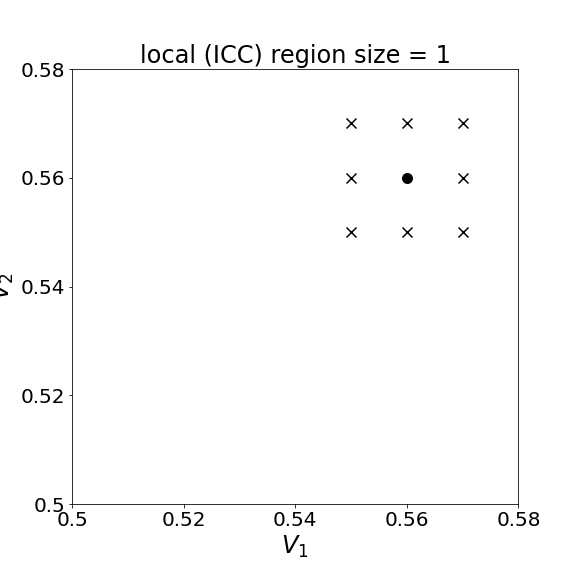
\includegraphics[width=0.3\textwidth]{images/local_size_1.png}
%     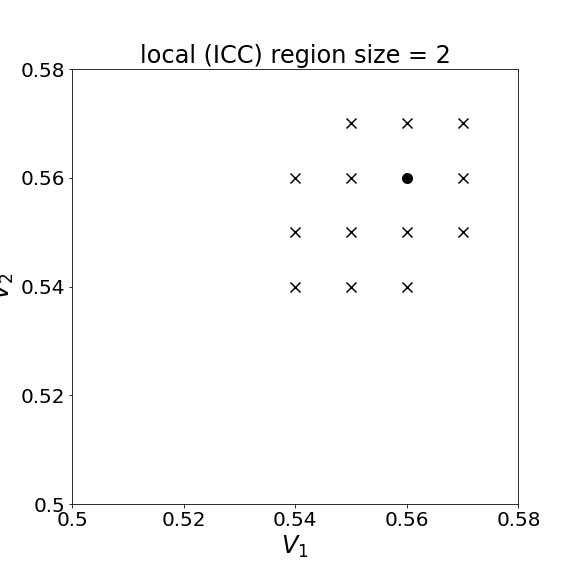
\includegraphics[width=0.3\textwidth]{images/local_size_2.png}
%     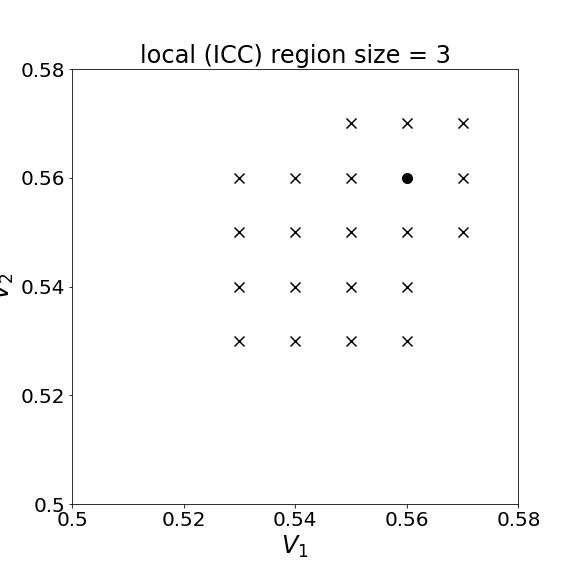
\includegraphics[width=0.3\textwidth]{images/local_size_3.png}
%     \end{center}
    
%     \vspace{1mm}
%     \raggedright{\small {\sc Figure \refstepcounter{fig}\thefig\label{fig:sim1}:} We iteratively grow the local region of the discretized type space checked for downwards-sloping constraint violations. Notice that immediately adjacent (ICC) constraints are always checked ($\times$) when the local region increases in size around a point ($\bullet$).}
% \end{figure}


% Belloni et al. \autocite*{belloni2010multidimensional} use a plane-putting algorithm which works with a randomly chosen subset of incentive-compatibility (ICC) and Border (B) constraints at each iteration. They provide an efficient reduction in the growth in $T$ of the Border constraints (B) from $O(2^{T^J})$ to $O(T^J \log(T^J))$ \autocite[Lemma 10]{belloni2010multidimensional}. We adopt their solution to checking (B) constraints; however, our approach to checking (ICC) constraints involves iteratively growing the `local' region of the type space around each point $v$ in the discretized set of types $V_T$. We do two things. First, all the immediately adjacent points in the discretized type space are always checked for incentive compatibility. Secondly, downwards-sloping points in the discretized type space are also checked. Furthermore, the downwards-sloping region of the type space grows until all (ICC) constraints are ultimately satisfied. This procedure is illustrated visually in Figure \ref{fig:sim1}. Thus, for a fixed-size local region around each point in the discretized type space, we first satisfy \textit{local} (ICC) and (B) constraints as in the iterative plane-cutting algorithm of \autocite{belloni2010multidimensional}. Then we run the separation oracle with \textit{all} (ICC) and (B) constraints. We then restart the solver with any previously violated constraints, this time increasing the size of the local region around each point in the discretized type space. This procedure iterates until no constraints are violated. This modified version of \autocite{belloni2010multidimensional}'s algorithm is described in Algorithm \ref{alg:1}.

% \begin{figure}
%   \centering
%   \begin{minipage}{.7\linewidth}
%     \begin{algorithm}[H]
%     \caption{Iterative plane-cutting algorithm with local and downwards-sloping (ICC) constraints}\label{alg:1}
%     \SetAlgoLined
%     % \KwData{$x=1$}
%     % \KwResult{$y = x^n$}
%     % $\text{local_size} = 1$\;
%     $L = 1, S = \emptyset, A = \emptyset, \overline{OPT} = \infty$\;
%     \texttt{violated\_any\_icc} $\gets $ TRUE\; 
%     \While{\texttt{violated\_any\_icc}}{
%         \texttt{violated\_local\_icc} $\gets$ TRUE\; 
%         \While{\texttt{violated\_local\_icc}}{
%           $k = 1, A^k = A, S^k = S$\;
%           Solve the linear program associated with $S^k$. Let $OPT^k$ denote the optimal value.\;
%           Solve the separation oracle using only local (ICC) constraints in region $L$. Let $A^k$ denote all violated local (ICC) and (B) constraints.\;
%           \If{$A^k = \emptyset$}{
%             \texttt{violated\_local\_icc} $\gets$ FALSE\;
%             Break\;
%           }
%           Select a subset $I^k \subset S^k$ of inactive (ICC) and (B) constraints\;
%           \eIf{$OPT^k < \overline{OPT}$}{
%             $S^{k+1} \gets (S^k \setminus I^k) \cup A^k \cup A$\;
%             $\overline{OPT} \gets OPT^k$\;
%           }{
%             $S^{k+1} \gets S^k \cup A^k \cup A$\;
%           }
%           $k \gets k+1$\;
%         }
%         Solve the separation oracle using all (ICC) constraints. Let $A^*$ denote all violated (ICC) constraints.\;
%         \If{$A^* = \emptyset$}{
%             \texttt{violated\_any\_icc} $\gets$ FALSE\;
%             Break\;
%         }
%         $A \gets A \cup A^*$\;
%         $S \gets S^k$\;
%         $L \gets L + 1$\;
%     }
%     \end{algorithm}
%   \end{minipage}
% \end{figure}

% Our algorithm\footnote{For more details see: \url{https://github.com/jmemich/optimal-auction-multidim}} is written in Python 3.10 and uses Google's open source linear programming solver `GLOP' available in their \texttt{or-tools} package \autocite{ortools}.

